\chapter{Evaluation}
\label{evaluation}

This chapter is devoted to the description and discussion of three separate user
studies with the devices introduced in Chapter 2. Two studies were performed
with the original UCube device (one more informal than the other), while a longer,
more detailed study involved both the SnapCAD and PopCAD systems. We present the
procedure, results, and basic observations of each study in this chapter, and
discuss the results more thoroughly in the next chapter.

\section{UCube Pilot}

Early in 2011, shortly after the UCube prototype was complete, we conducted an
initial (and informal) pilot study with the UCube. Our participants were a group
of 12-14 year old middle school children from a local middle school multimedia
class. We had fourteen participants (predominantly Caucasian), consisting of
five girls and nine boys, who were divided into six groups (five groups of two,
one group of four).

\subsection{Procedure}

Participants were asked to model a sequence of five shapes of increasing
complexity using the UCube along with the companion software. The target shapes
were displayed on one half of a computer screen, while the UCube software
showing the live model was displayed on the other half (as in
\ref{fig:ucube_test1}). The first shape that participants were asked to model
was a straight vertical line; after this, the requested shapes were a diagonal
line, a cube, a triangular prism, and finally an irregular polyhedral object. No
shape required more than four towers to complete, and shapes were always
presented in the same order.

\begin{figure}[!ht]
\begin{center}$
\begin{array}{cc}
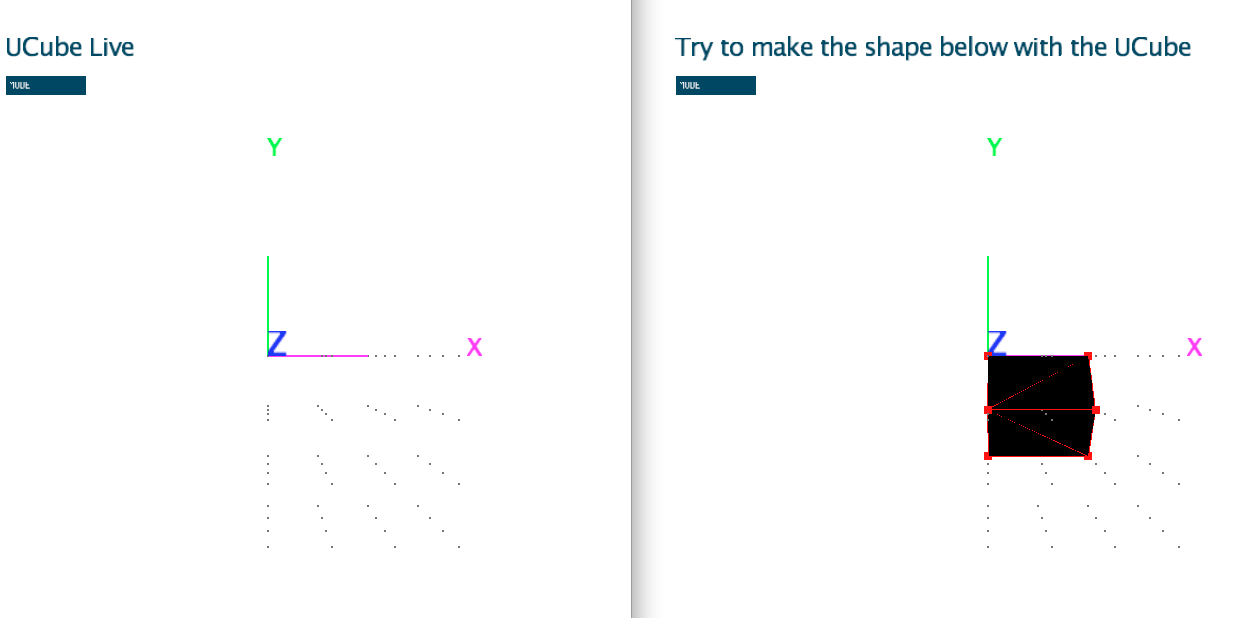
\includegraphics[width=.8\linewidth]{images/ucubescreentest}
\end{array}$
\end{center}
\caption{A screenshot of the testing setup, with the live output from the UCube
on the right and the target shape on the left.}
\label{fig:ucube_test1}
\end{figure}

Participants were instructed to place the tower on the board (but not shown
how), and were told that the software model could be rotated and filled in using
the keyboard and mouse, should that help them complete the task. The
participants were not given any hints as to how to complete the shapes and were
not told when they had the correct configuration (they had to indicate their
belief that the model was done). Participants were also instructed to ``think
aloud'' about their actions. The main purpose of the pilot study was to get an
initial impression of how the UCube would act as an accessible 3D modeling
tool - how well it could help ``3D novices'' overcome the ``2D bottleneck''.

\subsection{Results and Observations} 
Of the six groups who participated, four groups successfully modeled all five
shapes, one group ran out of time after three shapes, and one group finished one
shape, for a total of 24 of 30 possible shapes, or 80\%. Sessions lasted between
17 and 30 minutes. A variety of problem-solving strategies were observed during
testing, as the participants tended to treat the exercise as a sort of puzzle to
be solved. Simple methods equivalent to ``try and see'' were common, and seemed
to serve as a base point from which to draw conclusions about the relationship
between the 3D model and 2D on-screen representation (e.g. ``No, not there, up
one''). More sophisticated strategies were also observed: ``deconstructing''
more complex shapes into smaller, easier-to-model shapes (e.g. thinking of one
side of a cube as a square) was observed from several groups. Another popular
technique was to systematically match the on-screen perspective from the live
model with the shape they were attempting to model (e.g. ``Okay, first let's do
the top view, and then go from the side''). By orienting the two models
similarly, participants were able to make more accurate modeling decisions as
well as check their model against the on-screen shape. Counting distance in
terms of spaces on the board, between switches, or between dots on the screen
was also a very common technique of reasoning about and describing position. For
example, by counting that two vertices of a shape were separated by ``two dots
over and one down'' on the screen, subjects were able to count the distance out
on the physical UCube board. A few of the more mathematically-advanced
participants used terms such as ``axis'' and ``origin'' to orient themselves and
describe various positions on the board to their partners.
Another revealing observation in the pilot study was that, in the few instances
of mechanical failure (certain switches not lighting up, towers not plugging in
properly, or points not showing up on screen) the participants were still able
(with a high degree of certainty) to complete the assigned tasks. This appears
to indicate that, as opposed to arbitrarily moving the towers around until the
two sides of the computer screen looked the same, participants had formed a more
substantial mental model of the relationship between the UCube interface and the
2D representations on the screen. That opens the possibility that by performing
the embodied interactions necessary to operate the UCube, participants had
actually strengthened their understanding of how 3-dimensional space is
typically represented on a 2D screen. Although a small, informal study on its
own, this finding would strengthen the argument for using the UCube in an
educational setting to improve understanding of 3D space, as well as providing a
gateway for youngsters to move on to more complex modeling software.
While the variety of problem-solving techniques we witnessed is a testament to
the participants' ingenuity, it is also indicative of the fact that parts of the
UCube are not immediately intuitive. While none of the participants had trouble
understanding how to place the towers on the platform, the positions of the
towers and switches had to be reasoned out explicitly. It was common for groups
to clear the board of any poles when starting a new shape, even in cases where
an overlap of points or tower positions existed. Although most groups completed
all the shapes (or ran out of time), there were some expressions along the way
of the difficulty of the task (e.g. ``This is hard'', or ``This is like a
puzzle''). This indicates that design changes can be made in future iterations
to help clarify the correspondence between positions on the UCube platform and
the on-screen representation; for example, labeling the both the physical and
software grid with a simple alphanumeric system.
Despite these drawbacks as well as the inherent limitations of the UCube design,
these early results indicate a promising ability of youngsters to effectively
engage with the UCube interface. In fact, despite various levels of success in
completing the assigned tasks, the vast majority of participants exhibited a
high level of engagement with the UCube. For example, although the group that
completed only one shape seemed unmotivated to attempt to model the other
shapes, they continued to play with the interface and observe the results, even
stating ``this is fun'' and ``I like the switches''. Participants also saw
potential uses for the UCube outside of the specific exercise we assigned.
Comments (unsolicited) included, ``you should use this to teach geometry'' and
``you could make this a puzzle game''. At the very least, these early results
indicate that the majority of participants were able to take a 2-dimensional
representation on the screen and model its 3-dimensional equivalent using the
UCube, a very encouraging result in our eyes, prompting refinement of the UCube
software and hardware as well as further user study, as we explain below.

\section{Further UCube Study}

Early in 2012, we conducted an IRB approved follow-up user study of the UCube
with a group of 11-13 year olds. The group consisted of ten participants, eight
boys and two girls, from a local middle school multimedia class. Each
participant was individually led through two separate exercises (outlined below)
using the UCube.

\subsection{Procedure: Modeling}
Participants were handed a 3D-printed shape (modeled and printed from the UCube)
and were instructed to attempt to model the shape using the UCube. The
participant was initially allowed to hold the shape for approximately 10
seconds, after which they would hand the shape back to the facilitator and
attempt to model the shape from memory. Participants were instructed that they
may ask to hold the shape again, at which point they were allowed to hold it
throughout the duration of the modeling task. Additionally, users were
instructed that they had the option to skip a shape and return to it at a later
point in the exercise.
The five physical shapes presented were: a cube, a tetrahedron, a diamond, a
``house'' (a cube with a pyramid on top), and a complex irregular polyhedron.
The models were presented to the user starting with the cube (as this was deemed
to be the most basic shape with regard to modeling complexity). To avoid an
ordering bias, we randomized the presentation sequence of the next four shapes
using an online random order generator. If, after skipping a shape and returning
to it, the participant was still having difficulty, we offered them the
opportunity to attempt modeling the shape with the help of the UCube software,
the effects of which are discussed in the results section. Participants were
given a total of 25 minutes for the modeling exercise. We recorded, but did not
limit the modeling time per shape, only the total time for all five shapes.

\subsection{Procedure: Matching}
Participants were instructed to face away from the UCube while the facilitator
modeled a set of lights on the UCube corresponding to one shape among a set of
physical models laid out on the table next to the UCube.
Once the lights on the UCube were set up, the participant was instructed to turn
around, and indicate which physical object they thought the set of lights on the
UCube corresponded to.
There were nine physical models presented on the table, and consisted of a cube,
a tetrahedron, the ``house'' shape, a diamond, a triangular prism, an elongated
hexagon, a parallelogram, a trapezoid, and an irregular polyhedron (see
\ref{fig:ucube_shapes} for a picture of all the models). The shapes were always
presented on the table in the same order and orientation to avoid discrepancies
in perception or association.
Of the nine shapes, the participants were asked to match five of them (the cube,
the triangular prism, the parallelogram, the elongated hexagon, and the
trapezoid). Thus, only the cube was presented in both the matching and modeling
exercises. As with the modeling exercise, the cube was presented first, with the
remaining four shapes presented in a computer-generated randomized order.
Participants were given a total of ten minutes for the matching exercise,
corresponding to two minutes per shape, and were instructed to think aloud
during the process.

\begin{figure}[!ht]
\begin{center}$
\begin{array}{cc}
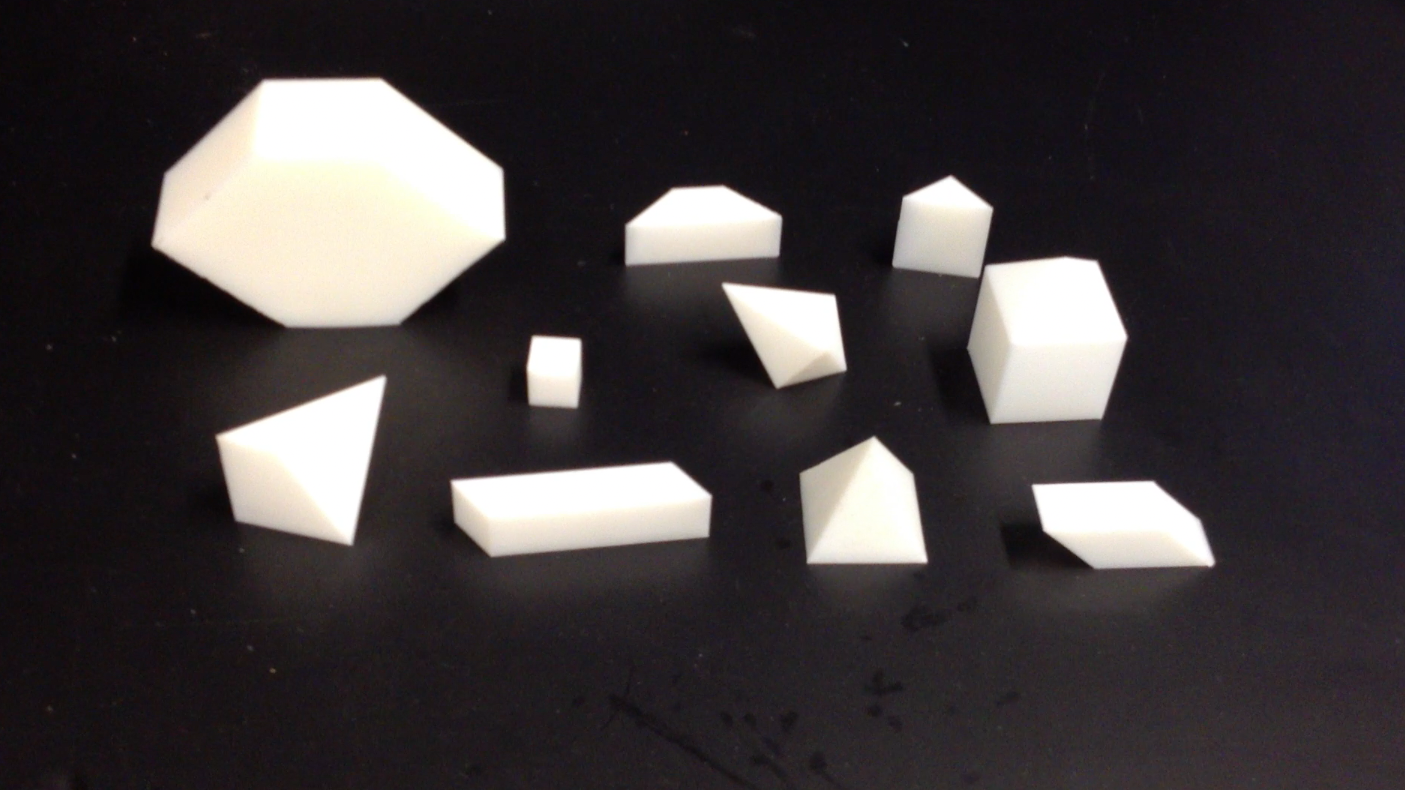
\includegraphics[width=.8\linewidth]{images/ucube_shapes}
\end{array}$
\end{center}
\caption{The nine models used during the user study:
a diamond, trapezoid, parallelogram, cube, elongated hexagon, irregular 
polyhedron, triangular prism, tetrahedron, house.}
\label{fig:ucube_shapes}
\end{figure}


\subsection{Results} 
While many established forms of 3D modeling systems can be confounding and
operationally too complex for a child to navigate, the UCube was positively
received and system instruction was accomplished with just a minor introduction
and demonstration (system instruction and demonstration lasted approximately 2-3
minutes). We found this first instance of system comprehension to offer some
validation that the UCube worked well as a user-friendly 3D modeling device.
This section will detail the outcome of both the modeling and matching tasks
performed.

\subsubsection{Exercise 1: Modeling} 
Modeling occurred under three conditions: recreate the object from memory,
construction of the object while it was in the participant�s possession, and
modeling the shape with the help of the UCube software. Overall, 21 of 50 shapes
were completed from memory, 12 of 50 were completed while holding the shape, and
a further 8 of 50 were completed with the aid of the UCube software, for a total
of 41 out of 50 shapes modeled successfully (82\%). Of the nine missed shapes,
seven were of the same shape, the complex polyhedron. The remaining two misses
were from the same participant, who ran out of time before completion.
Of the ten participants, eight were able to recreate the cube from memory,
whereas only four were able to recreate the diamond and the tetrahedron from
memory. Half of the participants constructed the house from memory, and no
participants were able to complete the irregular polyhedron from memory.
However, once shown the software the majority of the participants found the
modeling task significantly easier to perform. The irregular polyhedron was by
far the hardest shape and was only able to be completed by three of the ten
participants either after continued possession of the shape or using the
software.

\begin{figure}[!ht]
\begin{center}$
\begin{array}{cc}
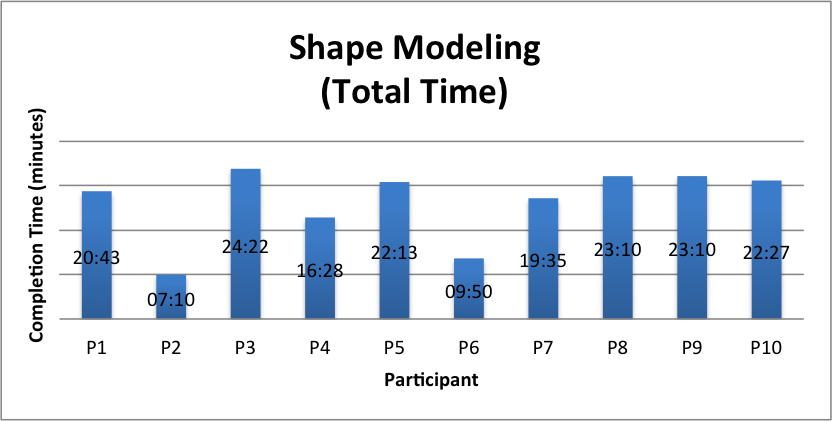
\includegraphics[width=.47\linewidth, height=1.75in]{images/modeling1}&
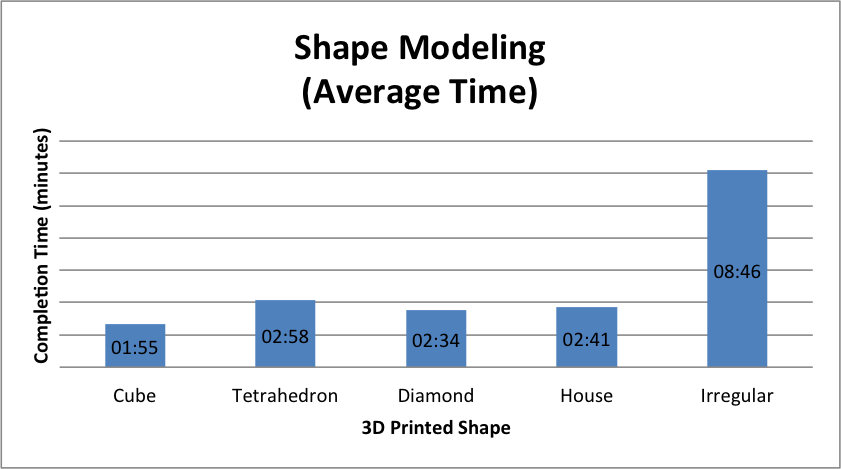
\includegraphics[width=.47\linewidth, height=1.75in]{images/modeling2}
\end{array}$
\end{center}
\caption{Results of the modeling task, showing total modeling time spent per
participant (left) and average modeling time spent per shape across
participants (right).}
\label{fig:modeling}
\end{figure}


The graphs in Figure \ref{fig:modeling} represent the total completion times per
participant (on the left) and average time per shape (right). Two exceptional
completion times were observed, where participants finished modeling all the
shapes in under 10 minutes. However, the majority of participants finished the
task in the 19-25 minute range. Only one of the participants ran out of time.
Once participants had been introduced to the software, 9 of 10 of participants
were able to complete all but the irregular polyhedron. It is interesting to
note that of the 10 participants, the child that had the most difficult time
modeling, the lowest shape completion rate, and the longest completion time
during the matching exercise was the youngest participant.


\subsubsection{Exercise 2: Matching} 
Out of 50 matching tasks (five per participant), all but three tasks were
completed in 20 seconds or less. Figure \ref{fig:matching} displays the total
time spent on the matching task per participant (left) and the average completion
times for each shape (right). No participant selected the wrong shape (a few
preliminary ``mis-selections'' were made that the participants quickly
corrected), and all participants completed the task in well under the allotted
10 minutes. The lack of errors in the matching task is highly encouraging as a
basis from which to reason about youngsters' abilities to perceive and reason
about convex hulls as a set of lit vertices in space, meaning that this kind of
3D modeling interface might be applied to other domains (e.g., as a cognitive
assessment tool, a puzzle game, etc.) with some optimism.

\begin{figure}[!ht]
\begin{center}$
\begin{array}{cc}
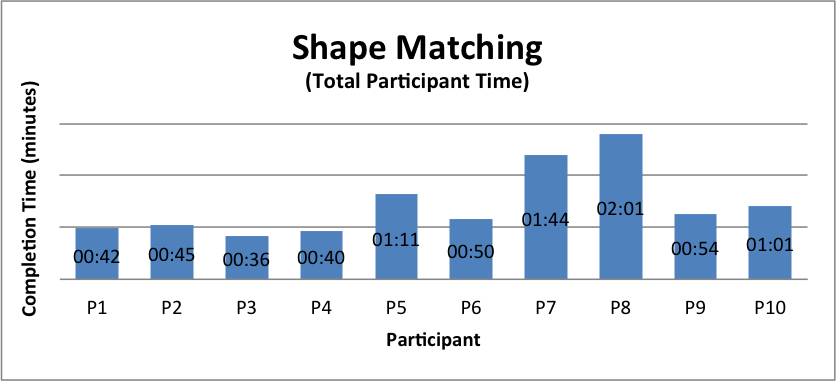
\includegraphics[width=.47\linewidth, height=1.75in]{images/matching1}&
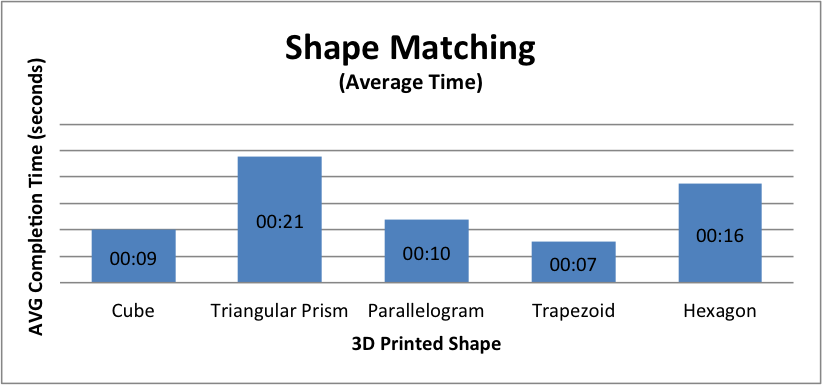
\includegraphics[width=.47\linewidth, height=1.75in]{images/matching2}
\end{array}$
\end{center}
\caption{Results of the matching task, showing total time spent per
participant (left) and average time spent per shape across
participants (right).}
\label{fig:matching}
\end{figure}


\subsection{Observations} 
Modeling trends as well as distinct modeling behaviors were documented in the
process. Common observations included building from the ground up (lowest
vertices first), building in the orientation that the object had been presented
in, not clearing the poles/lights from the UCube before starting to model a new
shape, and modeling a shape by breaking it up into discrete parts (e.g. a
participant building a house would commonly build a cube first and then add on a
vertex to the top; a participant constructing the diamond might combine two
opposite facing triangles).

\begin{figure}[!ht] \begin{center}$
\begin{array}{cc}
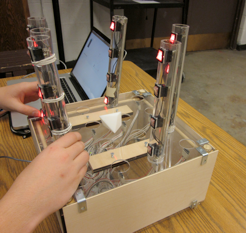
\includegraphics[width=.4\linewidth]{images/idc3}&
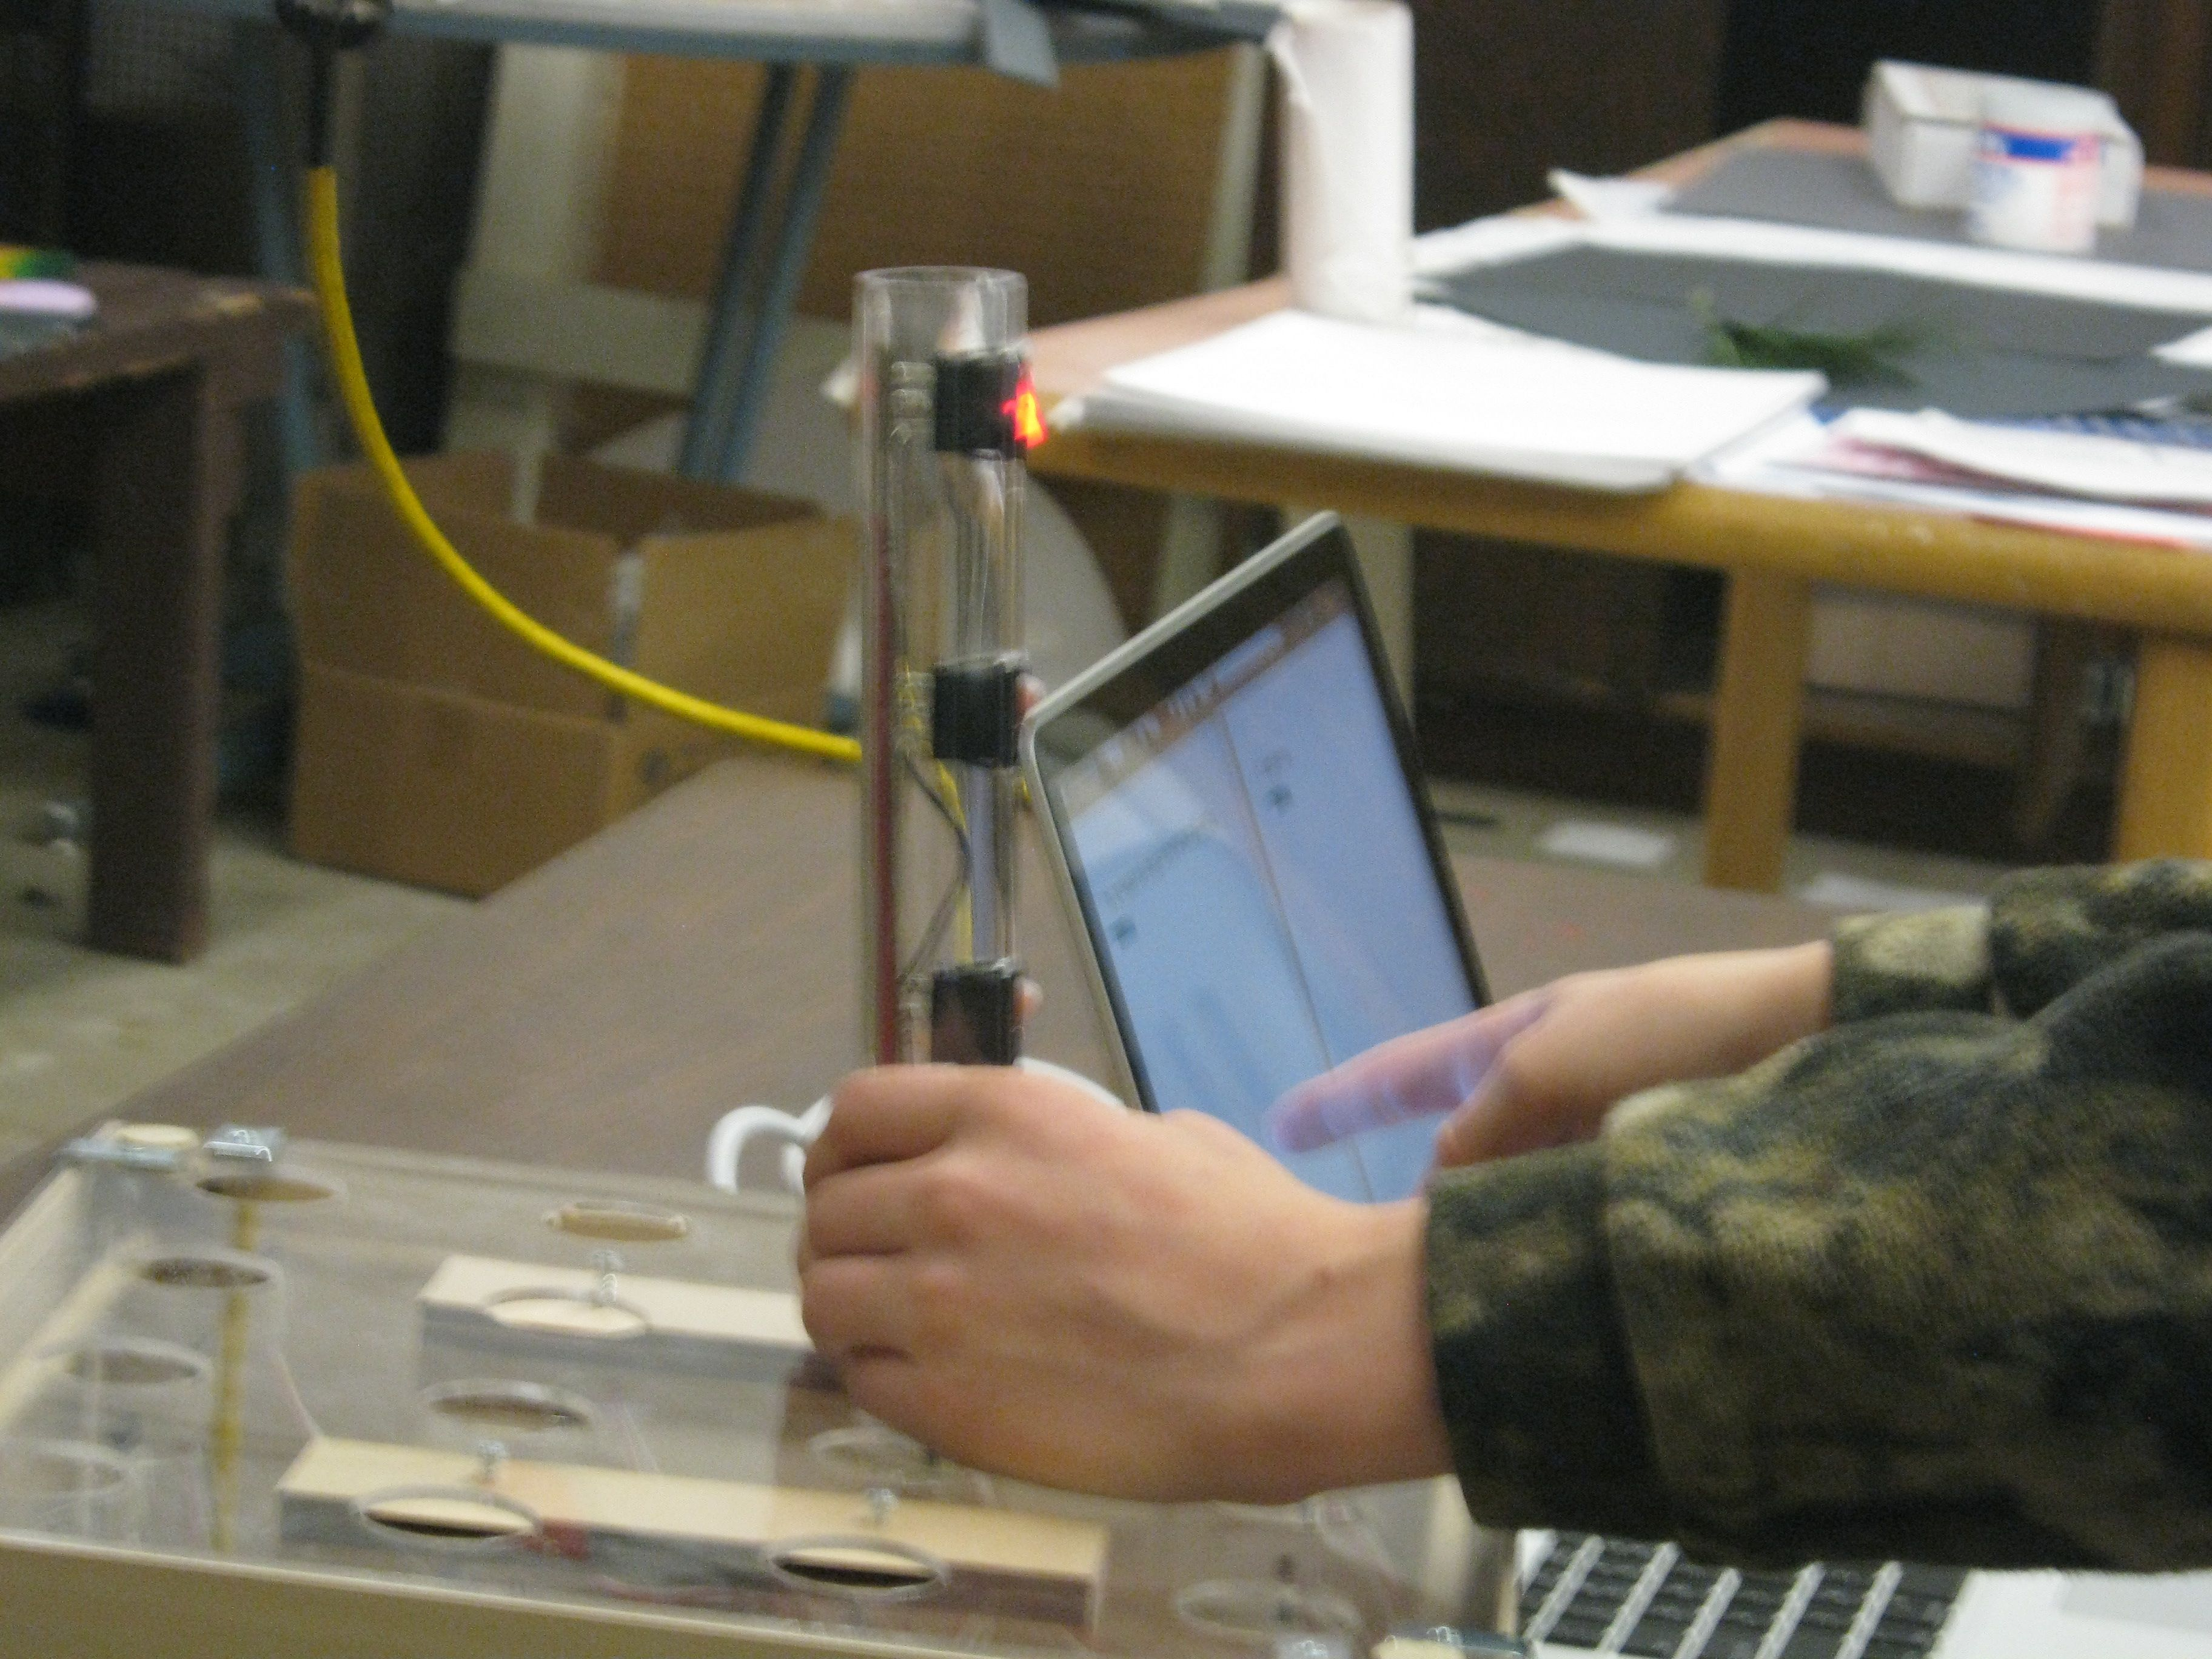
\includegraphics[width=.5\linewidth]{images/ucube1_user}
\end{array}$
\end{center}
\caption{Left: A participant using a strategy of
placing the physical model on top of the UCube while using both hands
simultaneously to manipulate the towers. Right: A user pointing at the software
representation of the shape with one hand, while manipulating the UCube
interface with the other hand.}
\label{fig:user_placedModel}
\end{figure}

Unique behaviors were exhibited in the modeling process as well, reflecting a
type of user specific construction-based problem solving. One participant used
their arm to connect the red lights of the UCube for shape definition. A few
participants oriented the object differently than how it had been
presented�typically this occurred for the modeling of those objects with a
pyramidal apex (tetrahedron, house, diamond). Apex formation was perhaps one of
the most difficult concepts for most participants to grasp, as it required them
to strategically align the base on a 3x3 grid so there was a middle plug for
them to create the apex. If participants were fixated on designing from a 4x4
grid then there was no center plug for them to create a midpoint. Some
participants ended up building an oblong polyhedron as opposed to a cube, or an
oblique polyhedron as opposed to an equilateral tetrahedron. Other observed
behaviors included a participant who modeled shapes by turning on lights for an
entire shape edge, as opposed to just the corners and a participant who built
shapes that were floating, as opposed to resting on the base of the UCube.
There were also some notable behaviors regarding physical and gestural actions
of the participants. Many participants modeled with both hands simultaneously,
placing towers and flipping switches without a clear preference for a dominant
hand. Participants would often gesture with their arms following an arc in
parallel with a face of the object they were currently modeling. This ``tracing''
behavior was also noticed when participants were holding a physical model and
tracing a side of the object with their fingertip, often while rotating the
object with the other hand. Finally, during object possession phase three
participants actually placed the 3D object on top of the UCube in the modeling
space while they reasoned out the construction (see
\ref{fig:user_placedModel} for an example). These gestural and ``embodied''
interactions with the UCube, combined with a high degree of modeling success
spurred us not only to create a more robust and expressive system (called -
SnapCAD - as detailed in Chapter 2), but to attempt to tease out the
relationships between modeling on these kinds of devices and the gestures and
speech produced when subjects were explaining their strategy in using the
devices. This eventually led to a comparative study using two new devices, two
new modeling modes, and introducing metrics to analyze some of the ``embodied''
aspects hinted at above.



\section{SnapCAD and PopCAD}

%- see
%http://silccenter.org/index.php/testsainstruments#MRT for the instruments, see
%http://www.spatialintelligence.org/publications_pdfs/Ehrlich\%20Levine\%20\%20Goldin-Meadow\%20\%282006\%29.pdf

Starting in early 2014 we conducted a study using both the SnapCAD and PopCAD
devices with a group of 11-18 year olds at a local drop-in enrichment program
that focuses on children from under-served and low socioeconomic communities.
Twenty participants enrolled in the study, consisting of 12 boys and 8 girls (no
one responded with other, although it was an option). We collected some basic
demographic information, including age, race, grade level, 3D modeling
experience, 3D printing experience, computer ownership and use, interest in
engineering, and how difficult they thought classes in school were. Parental
consent was obtained (and child assent given) for each subject in the study.

To present a snapshot of the demographic findings, then: the participants were
primarily of Latino or Hispanic descent, but also included those of
African-American, American-Indian, Asian, and Caucasian descent. Grade levels
ranged from 6th-12th, with an overall average of 7.9 (8.33 for boys, 7.75 for
the girls). Average age was 14 years, 1 month, 20 days (14 years, 6 months for
boys, 13 years, 7 months for girls). 18 of 20 participants had a computer at
home. Describing their comfort level using a computer on a scale from 1 to 10
(10 being most comfortable), the participants averaged 7.9 (8 for boys, 7.75 for
girls), with no scores below a 5. Of the participants who had a computer at home
(all but two of the subjects), two reported using it only a few times a year,
five used it a few times per month, four used it a few times per week, and five
reported using the computer everyday. Only three of the participants had any
experience with 3D modeling software. Interestingly, only two of the
participants had never heard of 3D printing before enrolling in the study, but
none of them had ever designed or printed anything using a 3D printer - further
underscoring the lack of available tools for novice designers. When asked about
their interest in engineering, only seven children (all boys) stated they were
definitely interested. However, only two children (both girls) stated that they
were definitely not. The rest (11 kids) stated that they were either ``maybe''
interested, or ``not sure''. When asked how difficult they felt school classes
were, six responded ``easy for me'', 10 said `somewhat easy for me', and four
responded ``somewhat hard for me'' (no one responded ``hard for me'').

\subsection{Procedure}

The study ran for seven weeks total, comprising several stages, the first being
a pre-assessment of spatial reasoning skills. The spatial reasoning assessment was
done using the ``Children's Mental Transformation Task'' developed by Susan
Levine (\cite{ehrlich2006importance} pp.1260-1261). In the task, participants
are shown two pieces of paper, side-by-side. One piece shows a 2D geometric shape,
split apart and rotated in one of several different ways. All shapes were
symmetrical either horizontally or vertically (or both), and thus split along
either a vertical or horizontal line of symmetry. Shapes were translated in one of four
different ways: (a) translated perpendicular to the line of symmetry (direct
translation), (b) translated and then moved diagonally apart (diagonal
translation), (c) rotated 45 degrees outward from the line of symmetry (direct
rotation), or (d) rotated and then moved diagonally apart (diagonal rotation).
The other piece of paper contained the geometric shape, recombined correctly,
along with three incorrect choices. In the study we conducted, participants were
given two sets of 10 shapes, one set as a pre-assessment before doing any
modeling, and another (completely different) set of 10 after completing the
entire study, as a post-assessment. Figure \ref{spatialTest} shows an example
instrument, with the four possible translations.

\begin{figure}[!ht]
\begin{center}
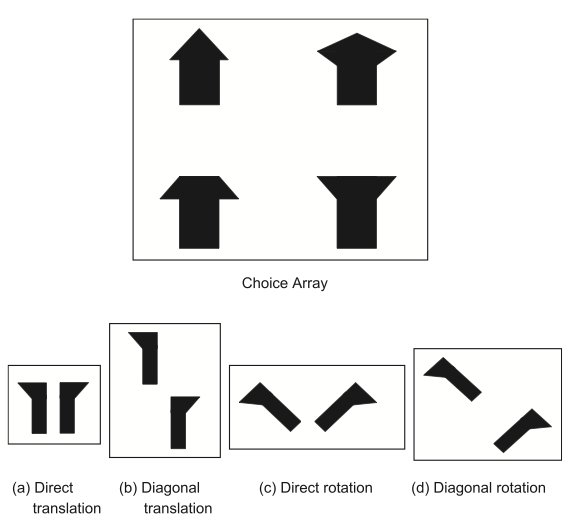
\includegraphics[width=.5\linewidth]{images/SpatialTestArray}
\end{center}
\caption{An example problem from the spatial reasoning exercise. The figure at
the top shows the choice array of four shapes, where the lower right figure is
the correct option. Examples (a) through (d) show the four different types of
translations found in the exercises - direct translation, diagonal translation,
direct rotation, and diagonal rotation.}
\label{spatialTest}
\end{figure}


After the pre-assessment, participants were split into two groups of 10 students
each - the selection alternated evenly based solely on order of participation -
with group A modeling first on the PopCAD and group B modeling first on the
SnapCAD (each device is described in Chapter 2). Each session begins with a
brief ($\approx$ one minute) introduction to the device, during which the
participant is told how to operate the device, but not what any of the software
buttons do, and given free time to become comfortable with the interface.
Participants were encouraged to explore both the interface, and the buttons in
the software that control the three primary modeling modes (convex hull, path,
minimal spanning tree).

Once the subject indicates that they are ready to move on (capped at 10
minutes), we move into a series of three modeling exercises that explore each of
the aforementioned modes. The basic operation and a brief explanation of each
mode were given to the participants as an introduction to each mode. Four
3D-printed models representative of each mode were presented to the user in an
order judged to be from least complex to most complex (and thus was the same for
each user), for a total of 12 modeling tasks across the three modes. 24 models
were used - one set of 12 was used across every user's first session
(independent of device), with a remaining 12 models used in every user's second
session. Figure \ref{3dModel} shows the two sets of models side-by-side.

\begin{figure}[!ht]
\begin{center}$
\begin{array}{cc}
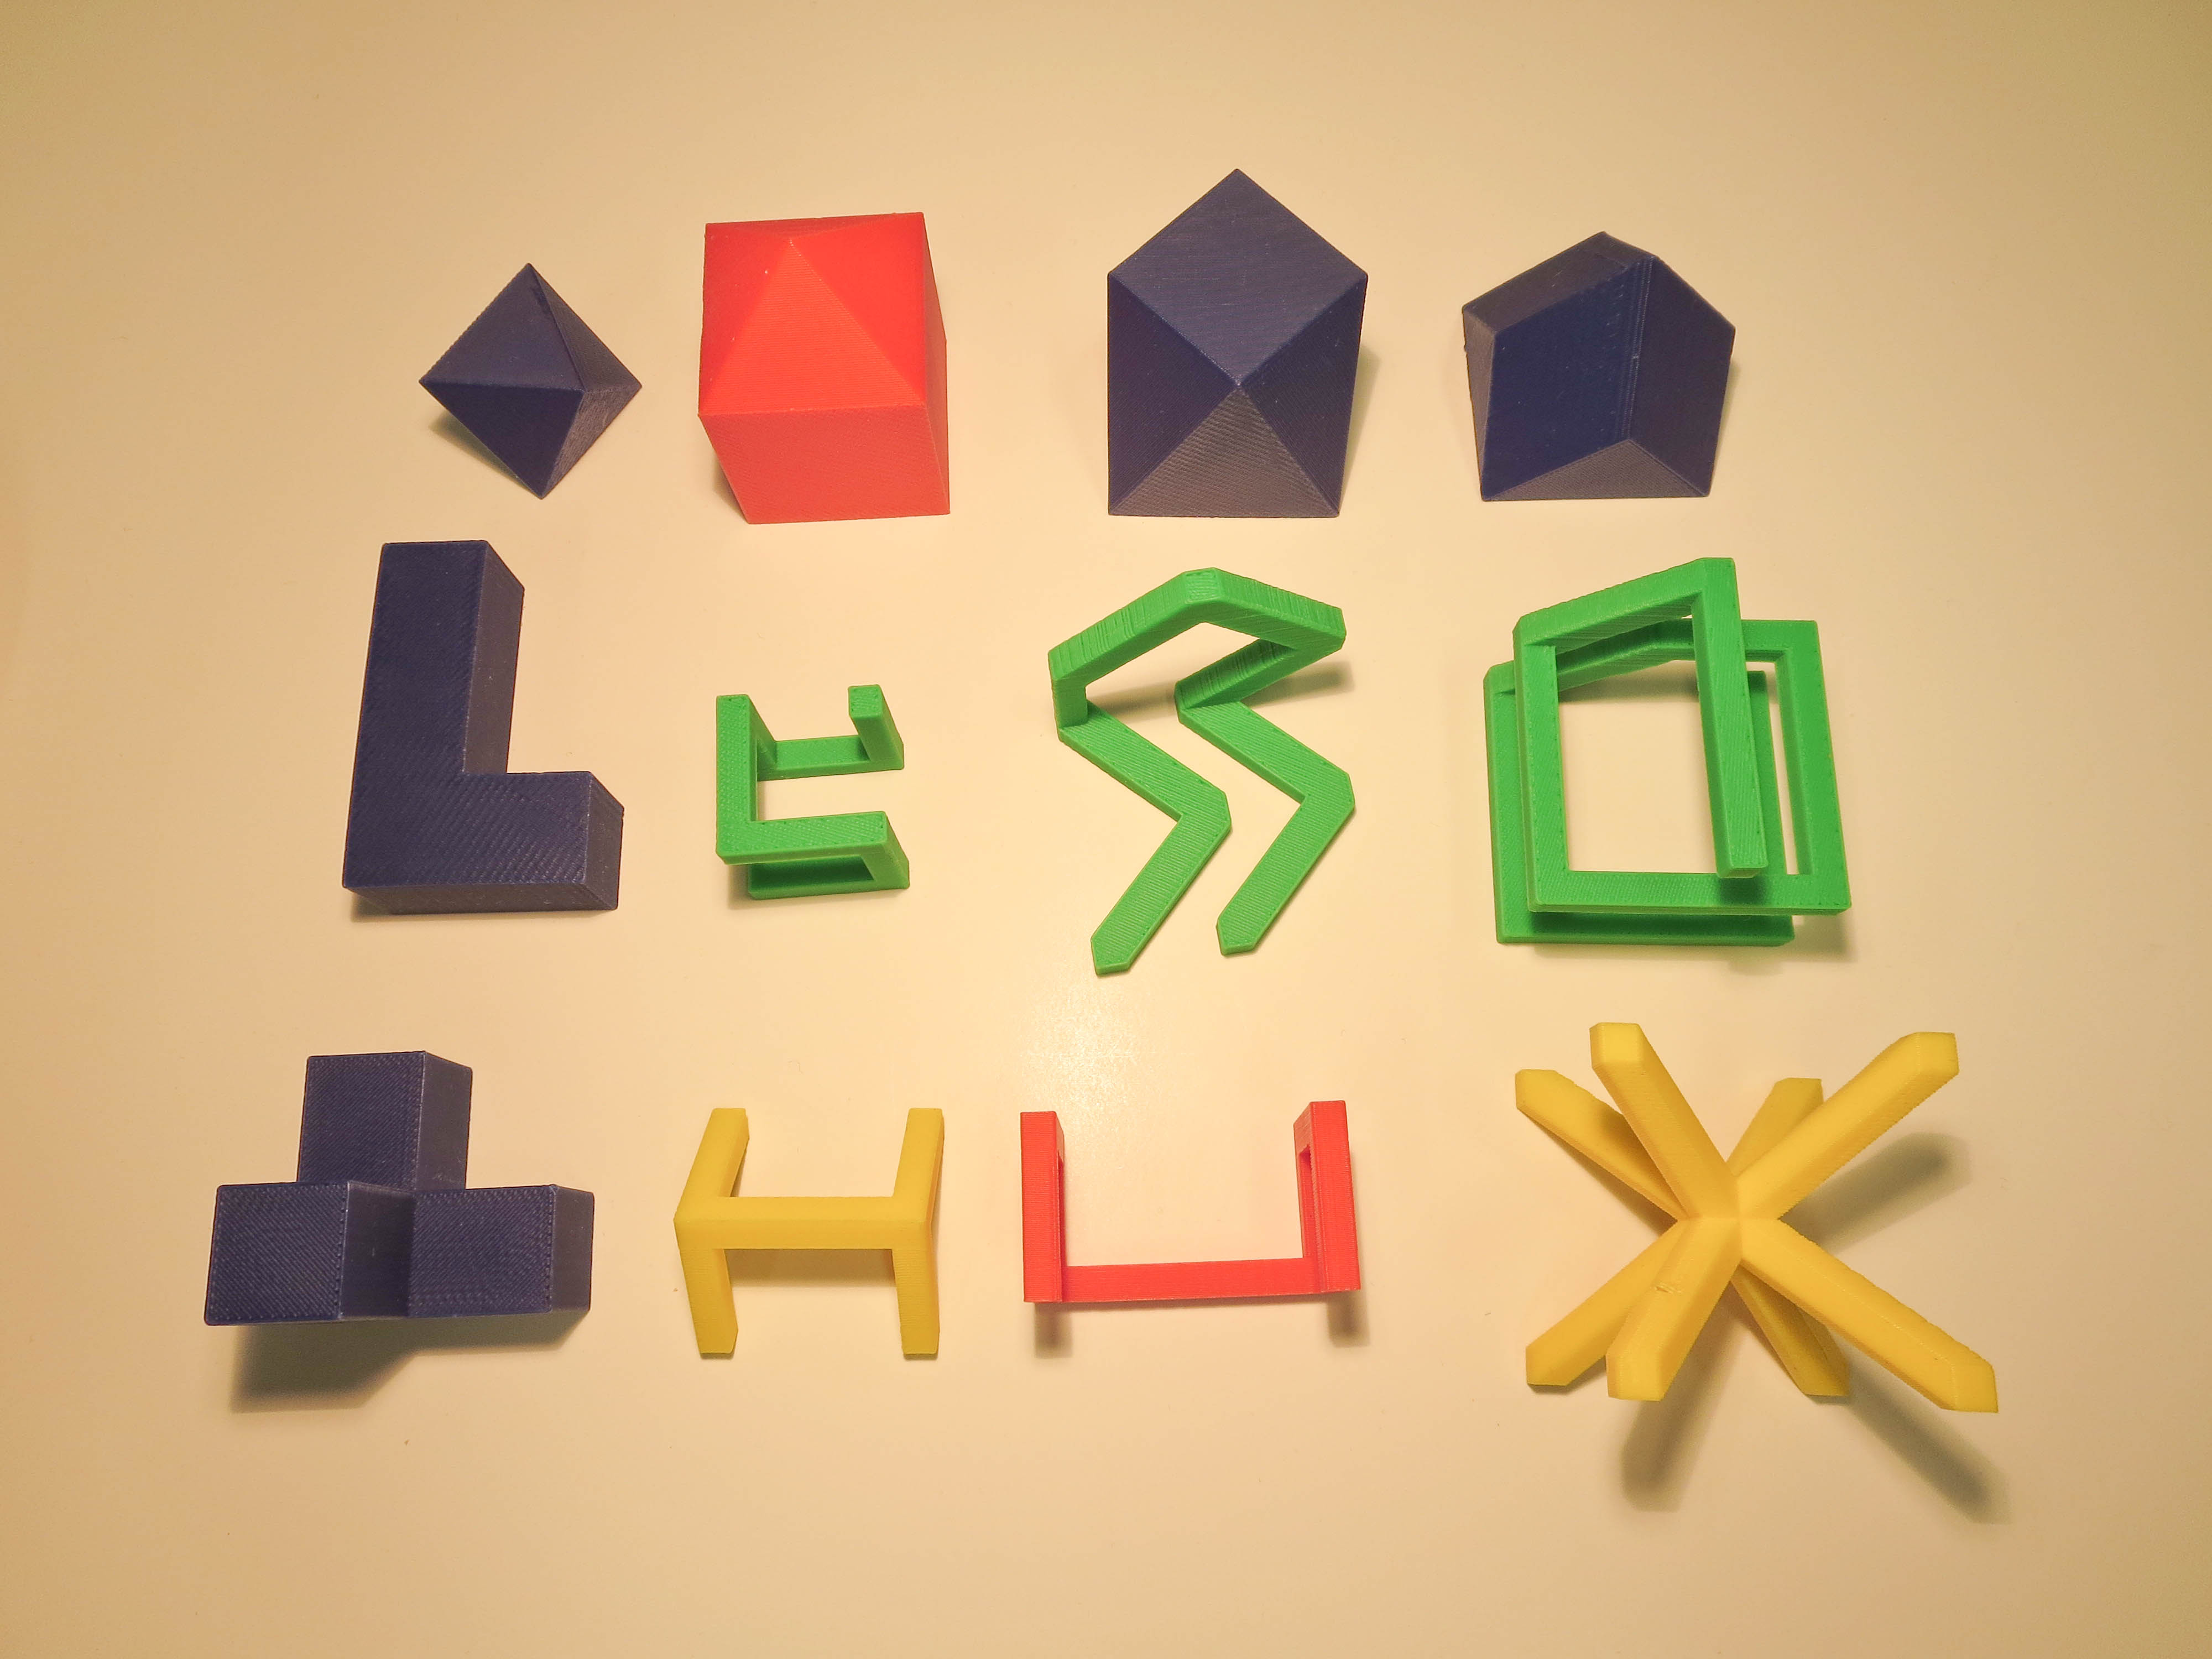
\includegraphics[width=.47\linewidth]{images/round1shapes}&
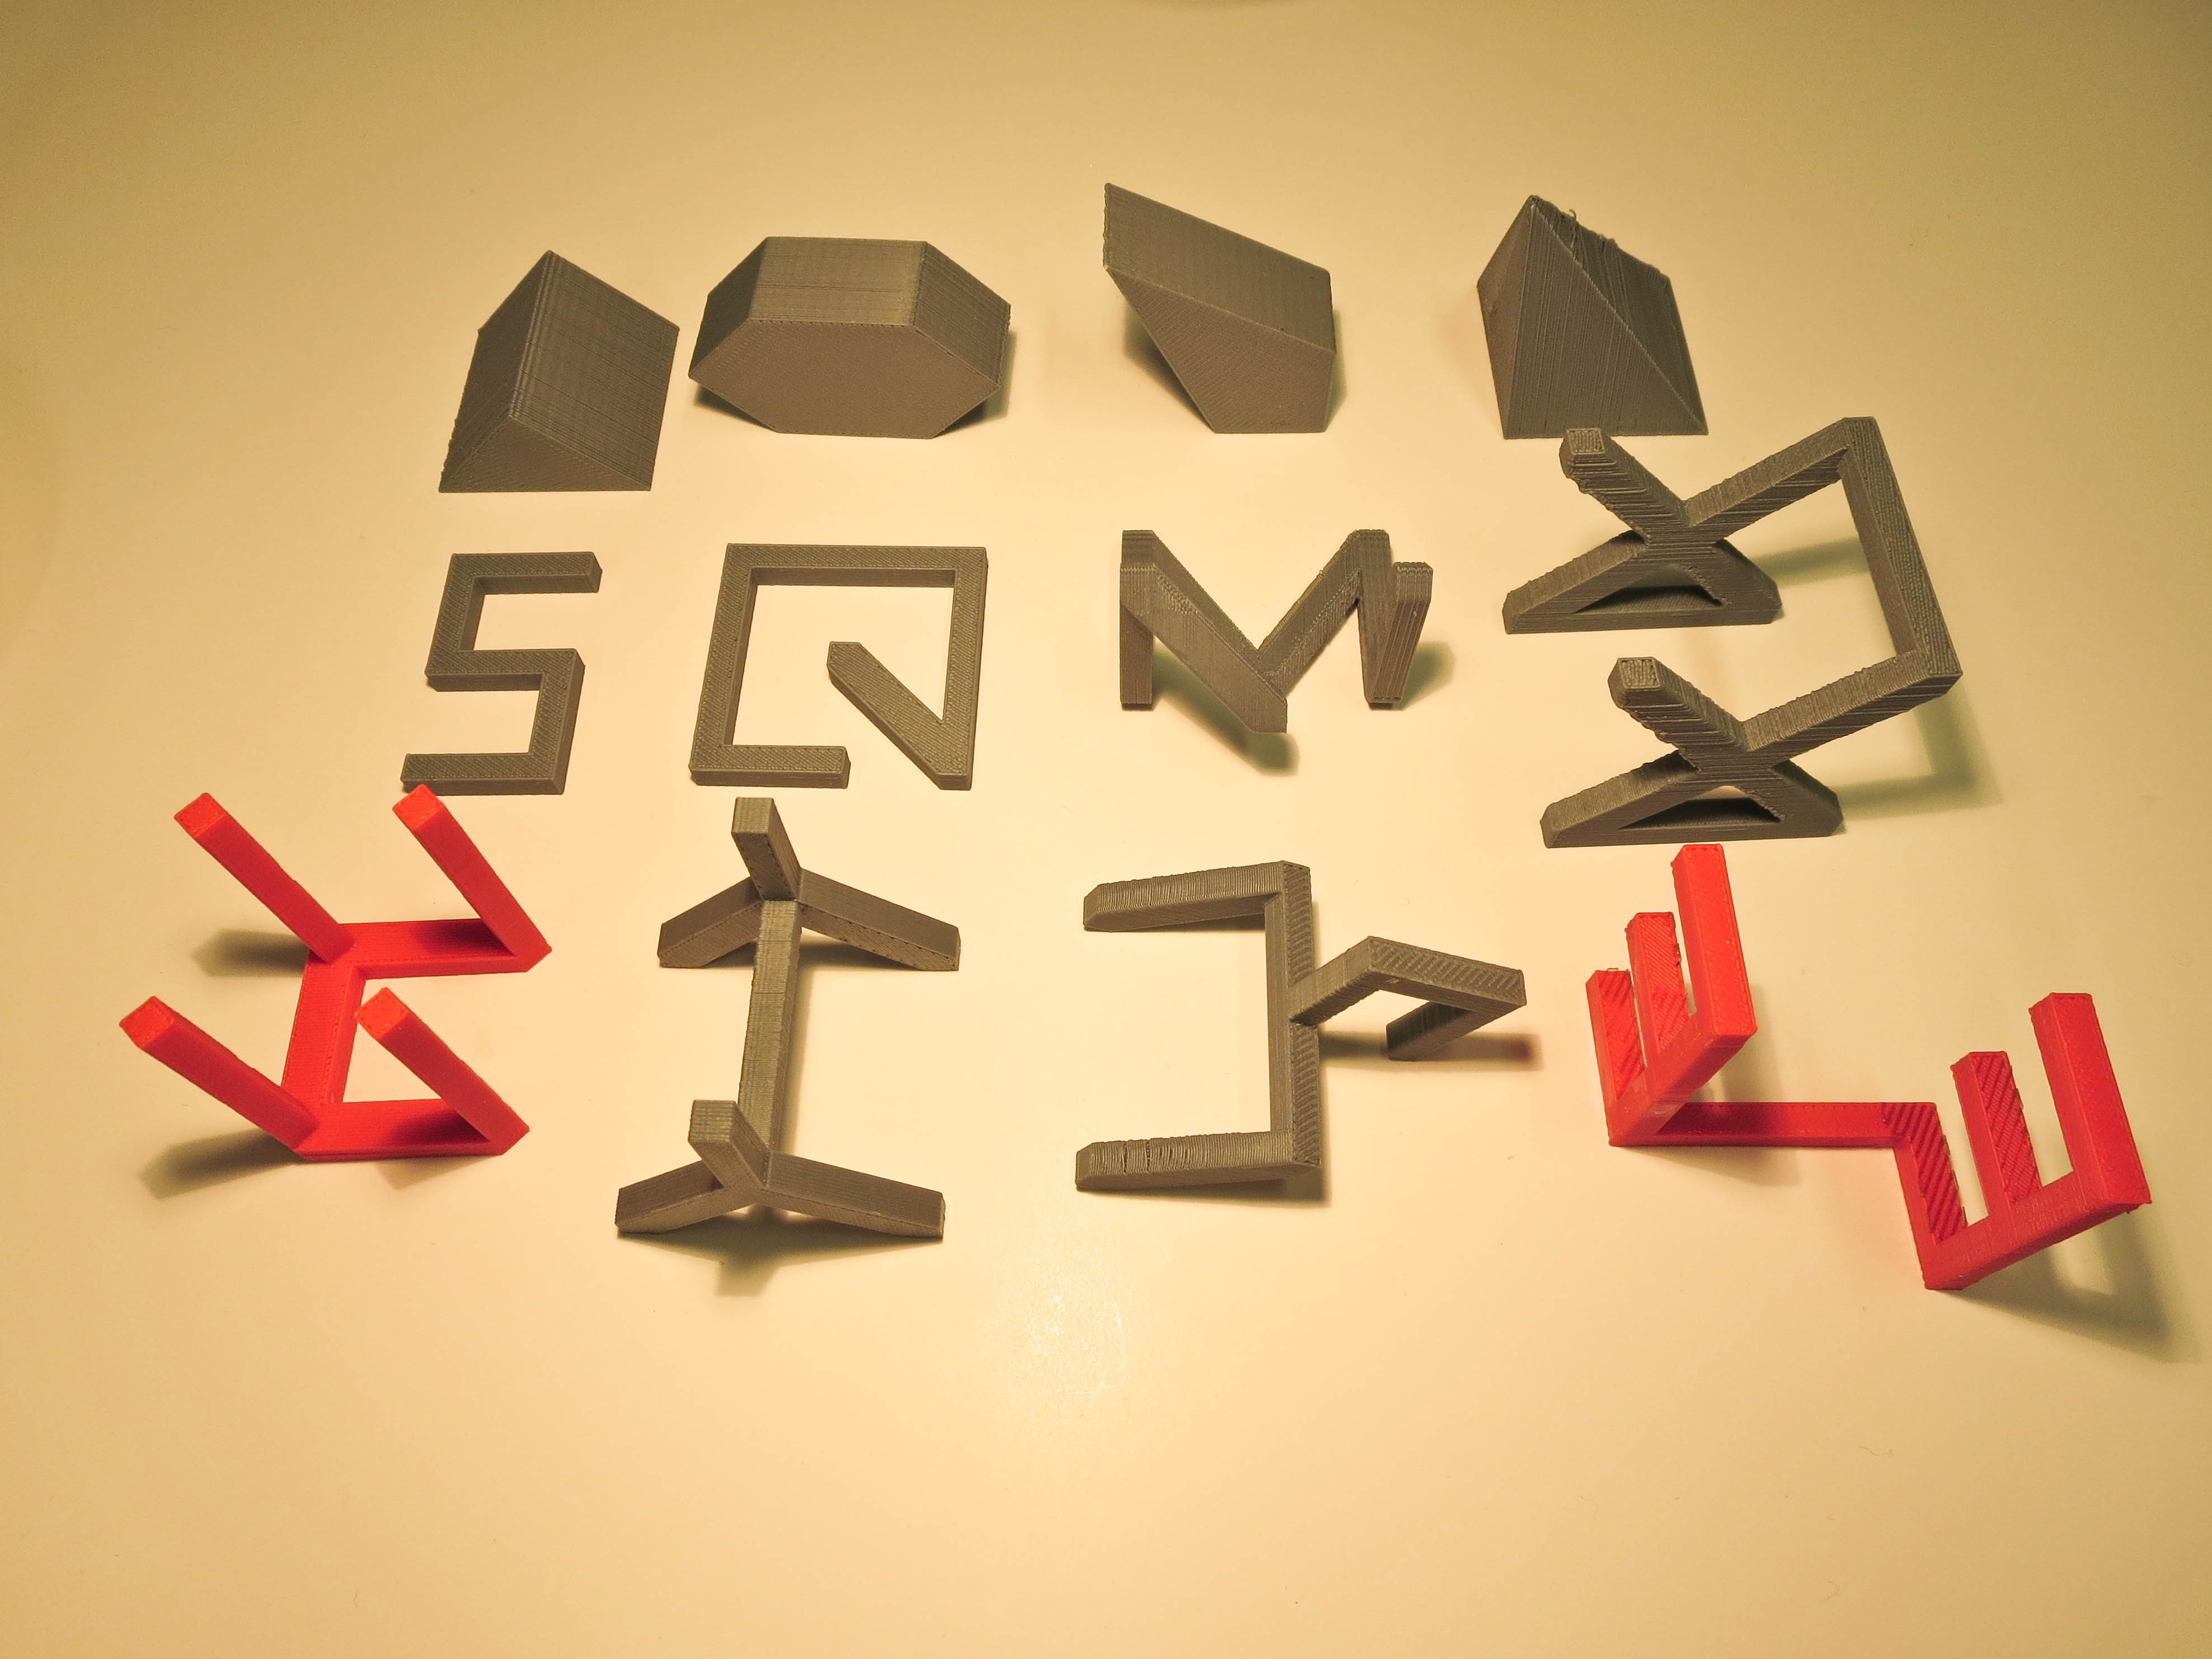
\includegraphics[width=.47\linewidth]{images/round2shapes}
\end{array}$
\end{center}
\caption{The two groups of 12 3D printed models used in the first session
(left) and second session (right). Each row is a different modeling mode (back
= convex hull, middle = path, and front = minimal spanning tree). The shapes
were presented in order from left to right as pictured above.}
\label{3dModel}
\end{figure}


The tasks that follow are the same for each device:

Tasks 1-3: Convex Hull Modeling, Path Modeling, Minimal Spanning Tree Modeling

Before each set of modeling tasks, the participant was given a brief demo of
how each modeling mode interprets the points from the device.  The user was
then presented with a series of four (4) plastic, 3D-printed models that were
modeled on the device using the current modeling mode. For each of these shapes,
the participant attempted to recreate the shape using the modeling abilities
of the device and the software. The user was be instructed to indicate when
they believe they have successfully recreated the shape, as well as to think
aloud about their modeling process. The time to completion (of lack thereof),
completion code, observational notes, and video were recorded. If the user
indicates modeling success, they shall be asked to explain their modeling
strategy for the purpose of logging gesture and speech data.

Task 4: Freehand Modeling

After the modeling tasks are complete, participants were invited to
``freestyle'' model an object of their choosing, using any of the three modeling
modes. By asking participants to think aloud about their intentions and thinking
processes during this exercise, we aimed to gain a deeper understanding of the
strengths and weaknesses of the system, as well as the thought processes and
engagement of the users in attempting to model a specific model of their own
choosing. These saved models were analyzed, based on which mode was used to
create them, complexity (based on number of points, faces, segments, and
symmetry), and whether the shape was ``exploratory'' or ``intentional'' (i.e.
was the end artifact a result of sort of happy accident, or the result of
intentional process to create a specific model).

For the first three modeling tasks (but not the freestyle modeling), time to
completion (or request to move on) was recorded, along with an outcome code. The
outcome was coded according to a set of conditions detailed below in table
\ref{modelingError}, and was developed upon analysis of the recorded video, in
an attempt to fit the sorts of repeated behaviors that were in fact observed.

\begin{table}[!ht]
\small
    \caption[Coding rubric used in analyzing modeling exercise outcomes.]{
	The coding used in analyzing the modeling exercise outcomes, based on
	observations from video taken during the study.}
    \begin{center}
    \begin{tabular}{| p{3.5cm} | p{1.0cm} | p{7.2cm} | } \hline
	$Category$ & $Code$ & $Definition$   \\ \hline
	Correct & C & A complete and correct modeling of the shape \\ \hline
	Error in recognition & E1 & The correct shape was modeled, but the user did not
	identify it \\ \hline 
	Error in belief & E2 & A belief that the modeled shape has been modeled
	correctly, when it has not \\ \hline 
	Error in implementation & E3 & User knew shape was incorrect, and gave a
	correct explanation \\ \hline 
	Error in strategy & E4 & Knew shape was incorrect, and did not know why or gave
	an incorrect explanation as to why \\ \hline 
	Error in proportion & EP & The general shape is correct, but the proportions in
	one or more dimensions is off (e.g. too tall, not wide enough, etc.) \\ \hline
	Incomplete & I & Participant ran out of time, gave up, or asked to move on \\
	\hline
	\end{tabular}
   \\ \rule{0mm}{5mm}
\end{center}
\label{modelingError}
\end{table}

Participants were asked to ``think aloud'' about their process, difficulties,
modeling choices, etc. In the case that the user believed they had correctly
modeled the shape (cases C and E2 in table \ref{modelingError}) they were asked
to explain their modeling strategy.\footnote{Cases E1,E3,E4, and I did not
provide the grounds from which to ask about modeling strategy and so were not
recorded.} Their explanation was videotaped and analyzed based on the coding
strategies laid out in ``The Importance of Gesture in Children's Spatial
Reasoning"(\cite{ehrlich2006importance}, p.1264), laid out in table
\ref{GcodingStrategy} below. The rationale for performing this analysis in based
in part on work by Ehrlich, Levine, and Goldin-Meadow
\cite{ehrlich2006importance}\cite{levine1999early}\cite{goldin2005hearing},
which suggests that the frequency of gesture and relationships between speech
and gesture act as a window into the learning state and performance of the
subjects.

\begin{table}[!ht]
\small
    \caption[Coding rubric for speech and gesture during user explanation of
    modeling strategy]{ The various coding strategies used in the video
    analysis of subjects' modeling strategy explanations. Borrowed and adapted
    from \cite{ehrlich2006importance}.}
    \begin{center}
    \begin{tabular}{| p{1.5cm} | p{4.2cm} | p{4.2cm} | p{4.2cm} |} \hline
	$Category$ & $Definition$ &   $Speech$ $Examples$  & $Gesture$ $Examples$ \\
	\hline Movement & Any indication of movement & ``Just slide them together and then it
	looks like that'' & Miming movement with the hands\\ \hline 
	Perceptual Features & Focus on a particular feature of the model & ``Because
	there is a little bend in here and a point thing here'' & Pointing to a
	specific feature on the model \\ \hline 
	Perceptual Whole & Any indication of seeing the model as a whole & ``It looks
	like an arrow!'' & Gesture indicating inclusion of the whole shape \\ \hline
	Vague & An expression of strategy that the coder cannot decipher & ``Because I
	looked at that and I looked at the differences'' & Waving gestures above the
	computer device that do not indicate any specific strategy \\ \hline 
	Other & Any strategy not listed above & ``And here is like half of it.
	But so and two halves make a whole'' & Using the hand to form a straight line
	through the middle of the whole shape to represent the line of symmetry
	\\
	\hline
	\end{tabular}
   \\ \rule{0mm}{5mm}
\end{center}
\label{GcodingStrategy}
\end{table}


The second session was similar to the first, with the subject using the device
not used in session one (no subject used the same device twice), and with 12 new
models. Once modeling on the second device was completed, users took a
second spatial reasoning assessment of an additional ten questions to help gauge
if any meaningful difference in spatial reasoning skills has occurred throughout
the study.

A slightly modified version of the software was used for the user study,
eliminating several of the functions not being evaluated for the sake of
presenting a clear interface for the users. The multiple hull modes, spline,
load, and save functions (described in Chapter 2) were eliminated, and the rest
of the graphical user interface was reorganized and streamlined. We
combined the three different .STL export buttons into a single export button
that handled all three modes, changed the order of the remaining buttons and
made them larger, and made the X,Y, and Z axis markings larger.

\subsection{Results}

This section reports on the results from our study, relaying our findings across
both sessions, genders, modeling modes, and spatial reasoning scores in an
attempt to tease out what conclusions, if any, we might make about the strengths
and weaknesses of our devices as well as how interacting with our devices
affected user's spatial reasoning abilities, 3D modeling skills, or congruence
between speech and gesture in explaining the cognitive learning state of the
user.

\subsubsection{Modeling Results}

In this section we will focus on delivering the results from the modeling
exercises. Users went through two sessions, modeling 12 shapes each time (four
shapes each using convex hull, path, and minimal spanning tree modes) for a
total of 24 exercises. For each modeling task, a result code was recorded per
the rubric shown in table \ref{modelingError}. One user dropped out of the study
(user six) before completing round one, leaving us to report on 19 users for the
first modeling session, ten of whom started on the PopCAD and nine of whom
started with the SnapCAD. A further three users did not complete session two,
leaving 16 users, seven girls and nine boys, who were split evenly over the two
devices in the second session (eight each on PopCAD and SnapCAD).

% \begin{table}[!ht] 
% \small
%     \caption[Modeling Results Overview]{This table gives the subject's age,
%     gender, and number of correctly completed modeling tasks during each of the
%     two sessions.}
%     \begin{center}
%     \begin{tabular}{| c | c | c | c | c | c | c |} \hline
% 	$User$ & $Age$ & $Gender$ & $Device$ & $S1$ $Score$ & $Device$ & $S2$ 
% 	$Score$\\\hline 
% 	1 & 14 & M & Pop & 11 & Snap & 9 \\ \hline
% 	2 & 12 & F & Snap & 6 & Pop & 8 \\ \hline
% 	3 & 15 & M & Pop & 6 & Snap & 3 \\ \hline
% 	4 & 13 & M & Snap & 4 & Pop & 5 \\ \hline
% 	5 & 12 & M & Pop & 5 & Snap & 6 \\ \hline
% 	7 & 15 & M & Pop & 12 & Snap & 11 \\ \hline
% 	8 & 12 & F & Snap & 4 & Pop & 8 \\ \hline
% 	9 & 18 & M & Pop & 8 & Snap & 3 \\ \hline
% 	10 & 14 & F & Pop & 12 & Snap & 10 \\ \hline
% 	11 & 17 & M & Snap & 9 & Pop & 12 \\ \hline
% 	12 & 12 & M & Snap & 4 & Pop & 7 \\ \hline
% 	13 & 13 & M & Pop & 9 & -- & -- \\ \hline
% 	14 & 14 & M & Snap & 1 & Pop & 5 \\ \hline
% 	15 & 12 & M & Snap & 1 & -- & -- \\ \hline
% 	16 & 13 & M & Pop & 12 & -- & -- \\ \hline
% 	17 & 13 & F & Pop & 11 & Snap & 9 \\ \hline
% 	18 & 17 & F & Snap & 8 & Pop & 12 \\ \hline
% 	19 & 11 & F & Pop & 4 & Snap & 3 \\ \hline
% 	20 & 13 & F & Snap & 0 & Pop & 5 \\ \hline
% 	\end{tabular}
%    \\ \rule{0mm}{5mm}
% \end{center}
% \label{modelOverview}
% \end{table}

\begin{table}[!ht] 
%\small
    \caption[Modeling Results Overview]{An overview of the modeling task
    results, broken down into session number, gender, device, and modeling
    mode.}
    \begin{center}
    \begin{tabular}{| c | c | c | c | c | c | c | } \hline
	& $Session$ $1$ & \% & $Session$ $2$ & \% & $Total$ & \% \\\hline 
	$Overall$ $Correct$ & 127/228 & 55.7\% & 116/192 & 60.4\% & 243/420 & 57.9\% 
	\\
	\hline $Girls$ & 45/84 & 53.6\% & 55/84 & 65.5\% & 100/168 & 59.5\%  \\ \hline
	$Boys$ & 82/144 & 57.6\% & 61/108 & 56.5\% & 143/252  & 56.7\%   \\ \hline
	$PopCAD$ & 90/120 & 75\% & 62/96 & 64.6\% & 152/216 & 70.4\%  \\ \hline
	$SnapCAD$ & 37/108 & 34.3\% & 54/96 & 56.3\% & 91/204 & 44.6\%  \\ \hline
	$Convex$ $Hull$ & 40/76 & 52.6\% & 38/64 & 59.3\% & 78/140 & 55.7\%  \\ \hline
	$Path$ & 48/76 & 63.2\% & 44/64 & 68.8\% & 92/140 & 65.7\%  \\ \hline
	$Tree$ & 39/76 & 51.3\% & 34/64 & 53.1\% & 73/140 & 52.1\%  \\ \hline
	\end{tabular}
   \\ \rule{0mm}{5mm}
\end{center}
\label{modelOverview}
\end{table}

Out of the 228 modeling tasks in session one, the group successfully modeled
127, or roughly 56\%. Those users who started with SnapCAD performed 37 of 108
tasks, or 34\%, while those using the PopCAD device completed 90 of 120 tasks
correctly, for a success rate of 75\%. Girls completed 45 of 84 tasks (54\%),
while boys correctly completed 82 of 144 tasks (58\%). Individual scores ranged
from 0 to 12 (perfect), with an overall overage of 6.68 correct shapes per user.
Average correct shapes per user was 4.11 for SnapCAD and 9.00 for PopCAD.

In session two, 116 of 192 (60\%) tasks were performed correctly, with SnapCAD
modelers correctly representing 54 of 96 shapes (56\%) and PopCAD modelers
completing 62 of 96 shapes, or roughly 65\%. Girls completed 55 of 84 tasks
(65\%) while boys completed 61 of 108 tasks for 56\%. Individual scores ranged
from 3 to 12 (perfect), with an average of 7.25 correct shapes overall, while
the average correct shapes per user was 6.75 for SnapCAD and 7.75 for PopCAD.


% \begin{table}[!ht] 
% \small
%     \caption[Session one modeling results per shape]{ This table shows the
%     number of correct models generated from a given shape, broken down by
%     device, gender, and average modeling time spent on the shape. Session one
%     results only.}
%     \begin{center}
%     \begin{tabular}{| c | c | c | c | c | c | c |} \hline
% 	$Shape$ & $Total$ & $PopCAD$ & $SnapCAD$ & $Average$ & $PopCAD$
% 	& $SnapCAD$ \\
% 	 & $Number Correct$ & $Only$ & $Only$ & $Modeling Time$ & $Only$ & $Only$
% 	 \\\hline 
% 	 Convex Hull 1 & 8 & 7 & 1 & 6:33 & 5:25 & 7:49 \\ \hline 
% 	 Convex Hull 2 & 13 & 9 & 4 & 4:34 & 3:03 & 6:15 \\ \hline 
% 	 Convex Hull 3 & 8 & 7 & 1 & 5:29 & 4:33 & 6:32 \\ \hline 
% 	 Convex Hull 4 & 11 & 7 & 4 & 4:52 & 4:31 & 5:14 \\ \hline 
% 	 Path 1 & 17 & 10 & 7 & 2:08 & 1:22 & 3:00 \\ \hline 
% 	 Path 2 & 14 & 9 & 5 & 4:39 & 3:24 & 6:02 \\ \hline 
% 	 Path 3 & 8 & 6 & 2 & 6:21 & 4:52 & 8:00 \\ \hline 
% 	 Path 4 & 9 & 7 & 2 & 4:12 & 1:56 & 6:43 \\ \hline 
% 	 Tree 1 & 12 & 8 & 4 & 2:10 & 1:10 & 3:17 \\ \hline 
% 	 Tree 2 & 8 & 6 & 2 & 2:25 & 1:08 & 3:51 \\ \hline 
% 	 Tree 3 & 8 & 5 & 3 & 3:11 & 1:29 & 5:04 \\ \hline 
% 	 Tree 4 & 11 & 8 & 3 & 4:24 & 3:12 & 5:43 \\ \hline
% 	 \em{Total} & 127 & 90 & 37 & 4:15 & 3:00 & 5:38 \\ \hline
% 	\end{tabular}
%    \\ \rule{0mm}{5mm}
% \end{center}
% \label{codingStrategy}
% \end{table}

The two bar graphs in \ref{ModelingTimes} show the average modeling times broken
out over device and gender (on the top) and modeling mode (on the bottom).
Modeling times were recorded from the time the user was handed the shape until
they indicated either that (a) they believed the model to be complete, or (b)
they gave up, wished to move on, or thought they were as close as they were
going to get (though they knew their model to be incorrect). 

\begin{figure}[!ht]
\begin{center}$
\begin{array}{cc}
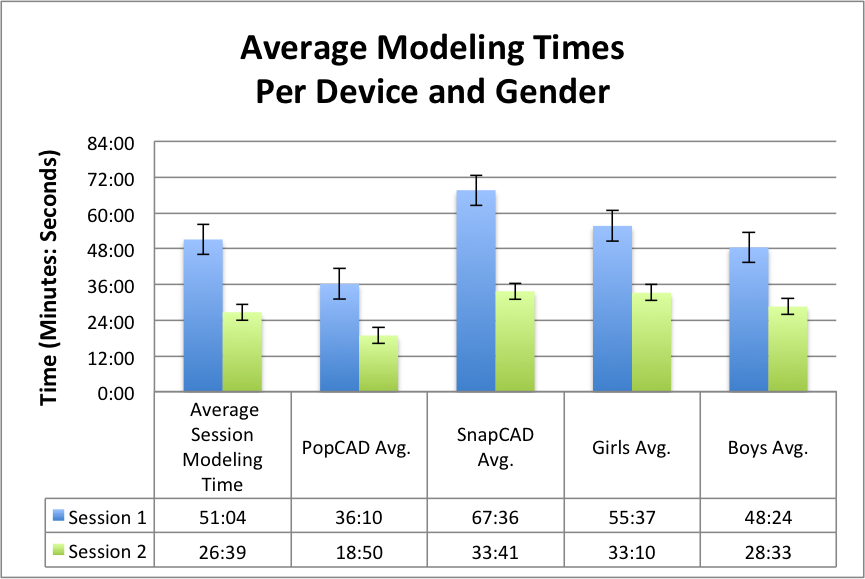
\includegraphics[width=.55\linewidth]{images/avgtimesmod} \\
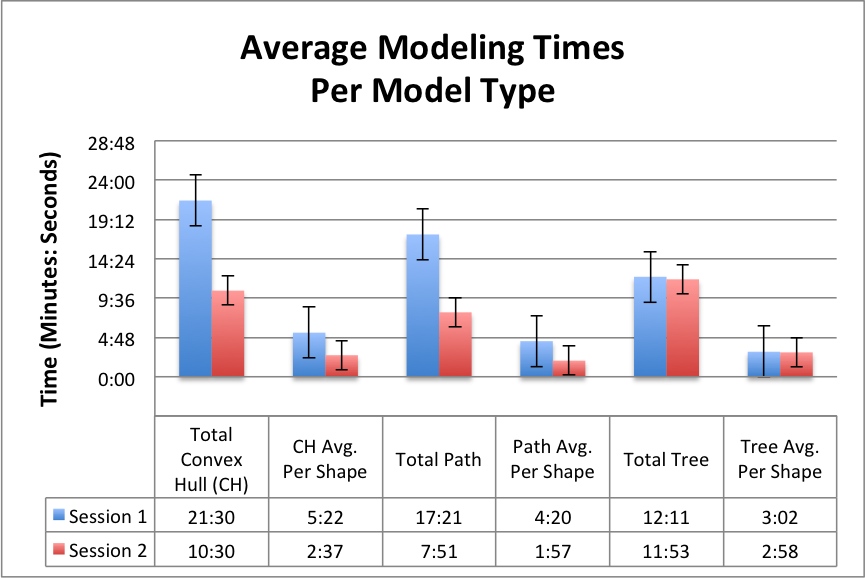
\includegraphics[width=.55\linewidth]{images/avgtimesmodeltype}
\end{array}$
\end{center}
\caption{The average recorded modeling times for each session, broken out (on
top) by device and gender, and (on the bottom) by modeling mode. Error bars
show standard error ($SE$).}
\label{ModelingTimes}
\end{figure}

We can easily pick out a few trends from these two graphs: average modeling
session time went down significantly in the second session, regardless of device
or gender, although boys took less time in both sessions, and the PopCAD seemed
to take less time overall in each session than modeling on the SnapCAD (although
interestingly, the SnapCAD modelers in the second round improved on their times
from modeling on the PopCAD in the first round). When examining mode types, we
see a similar trend of significantly decreasing modeling times in the convex
hull and path modes, but curiously, not in the tree mode where times improved in
the second session by only a few seconds. While the minimal spanning tree mode
took subjects the least amount of time (of the three modes) in session one, the
improvement in both convex hull and path modeling times left the spanning tree
with slowest overall and average modeling times in session two.
Seeing as the minimal spanning tree mode posted the lowest percentage of correct
shapes in both rounds (and thus overall), we might expect the ranking we
observed in round two, where average modeling times corresponded with the
overall percentage of correct shapes. It seems plausible that mastery of the
tree mode is slower to arrive than either the convex hull or path modes, and
therefore one extra session produced more dramatic results in the other modes
(convex hull and path modeling both improved by almost 7\% in session two,
minimal spanning tree by less than 2\%). 

% At the end of both sessions, the subjects were given the opportunity to model a
% shape of their own design, using any of the modes presented during the modeling
% exercises. Each participant modeled after the first round, and then were given
% the opportunity to create a different shape after the second round that they
% wanted printed out instead (most subjects stuck with their original model). The
% prints from the 16 participants who finished the study are shown in Figure
% \ref{UserShapesAll}.
% 
% \begin{figure}[!ht]
% \begin{center}
% 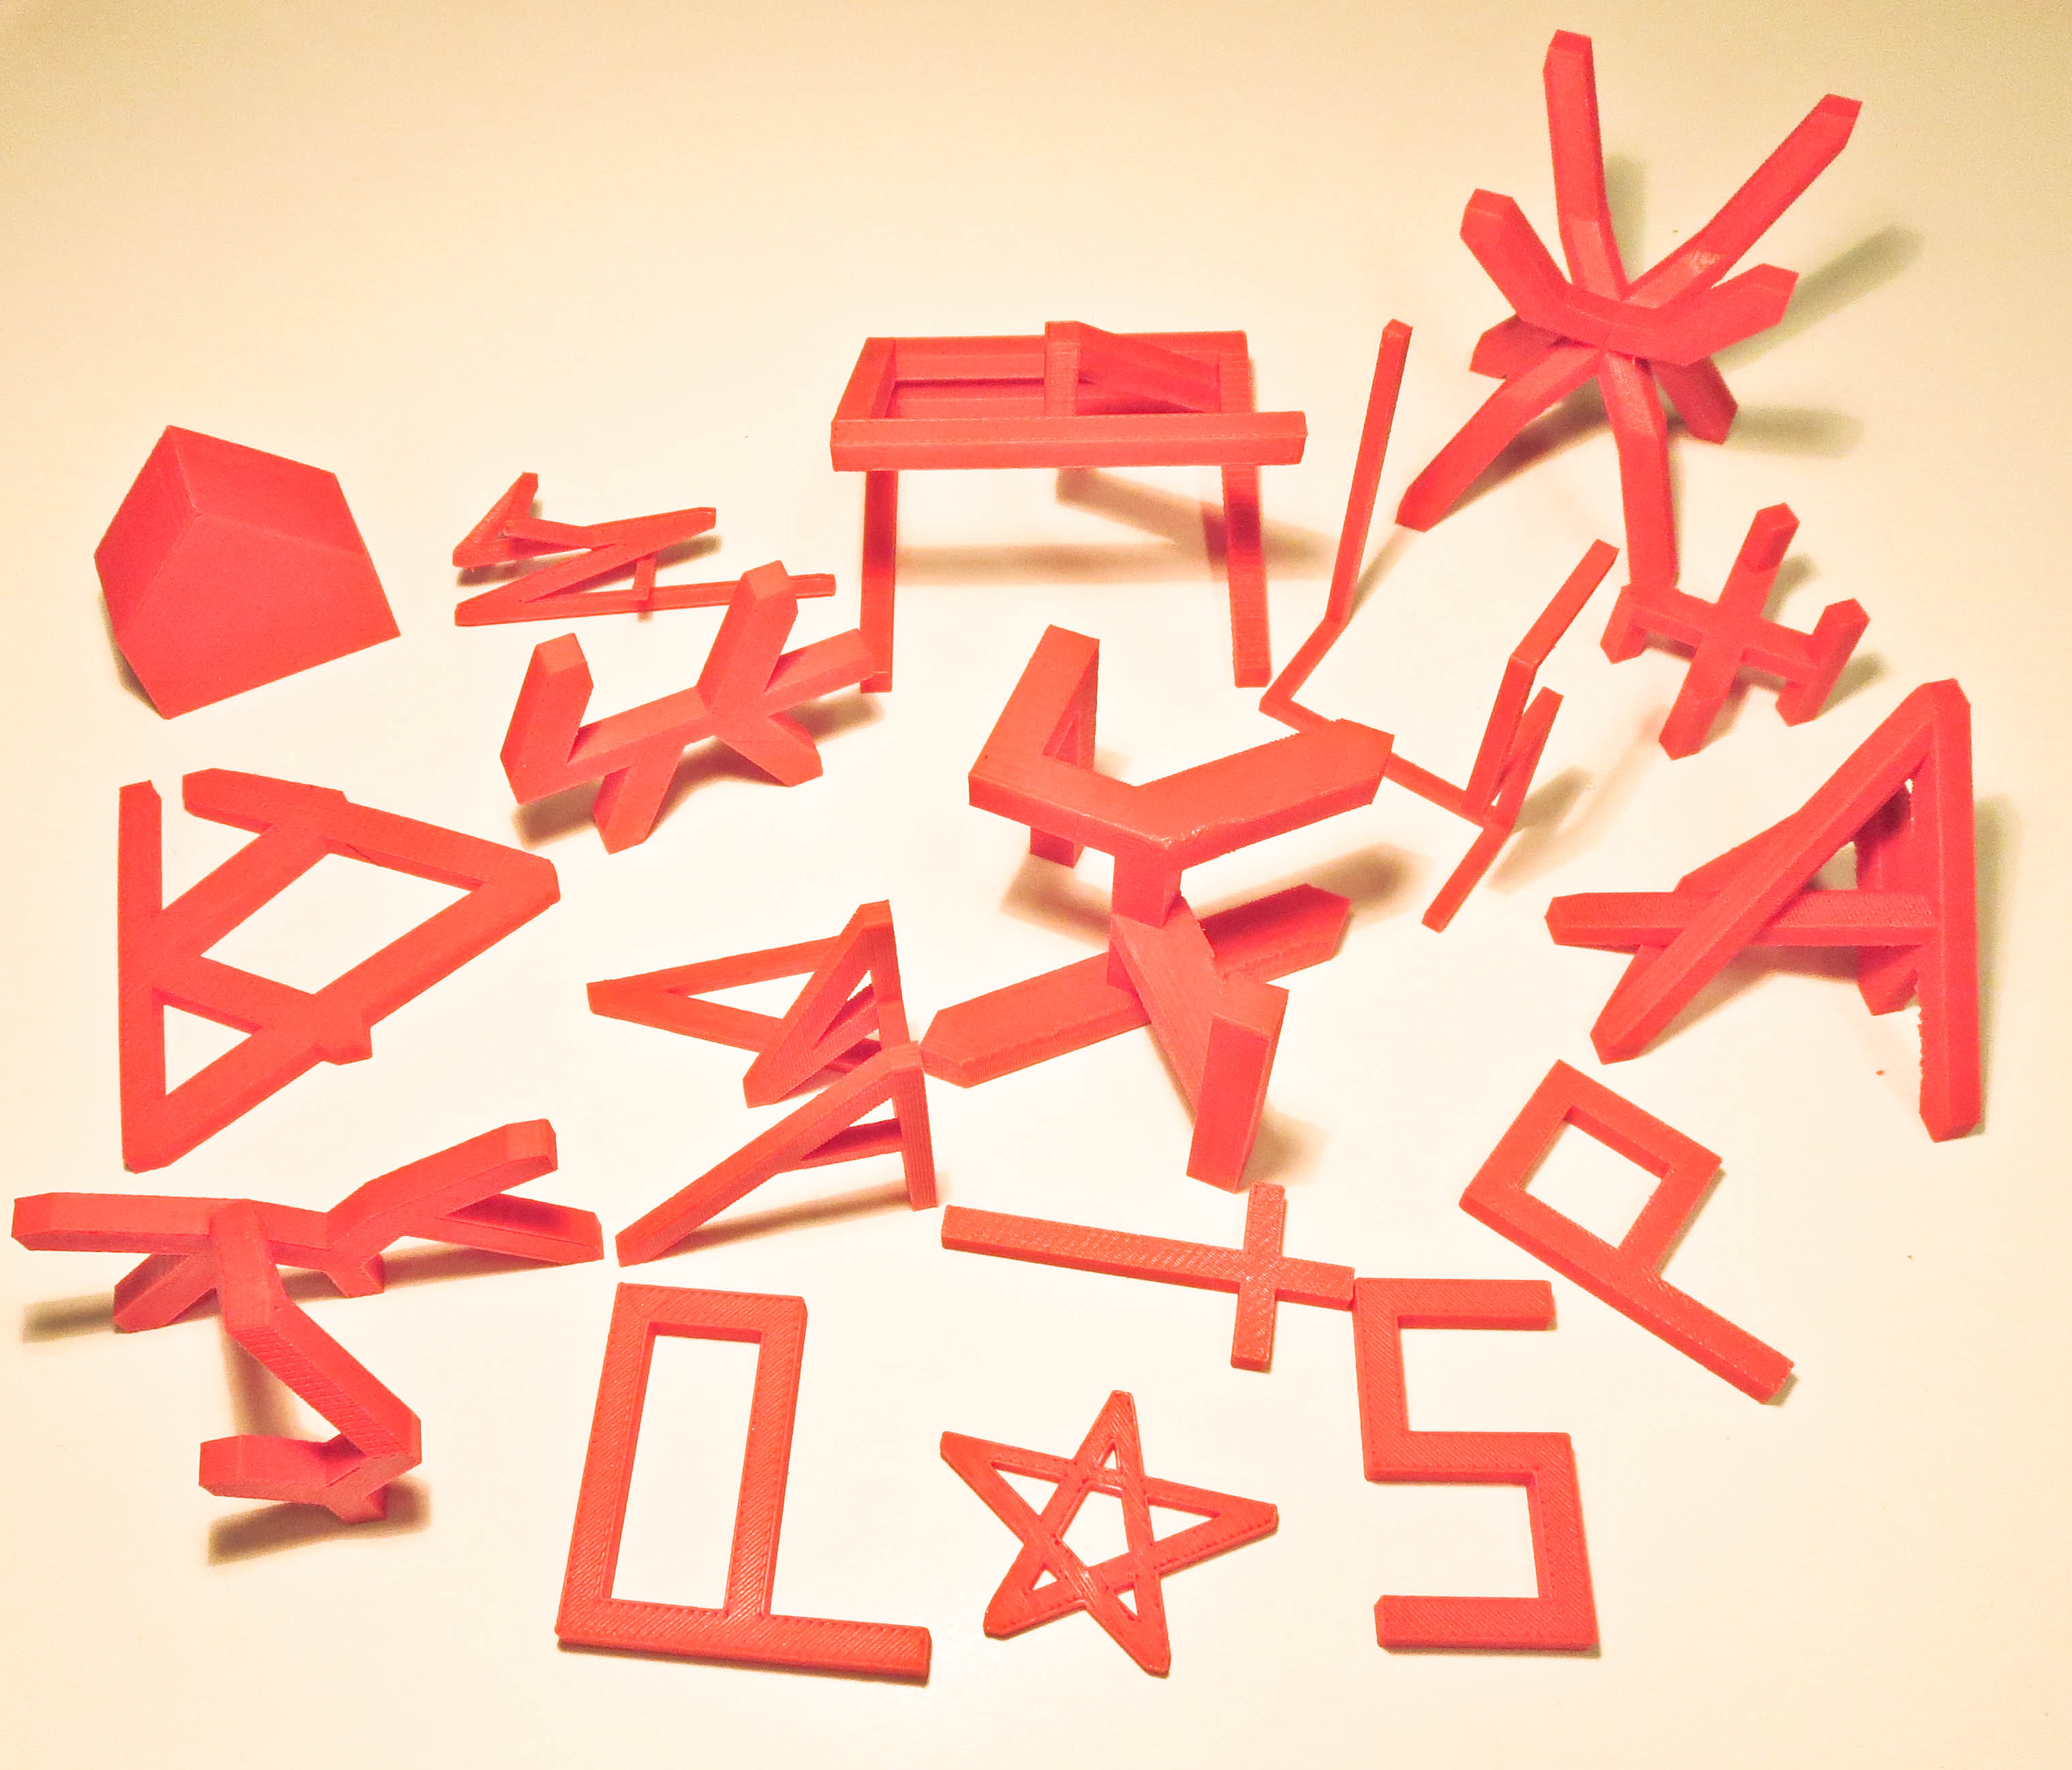
\includegraphics[width=.55\linewidth]{images/userShapesAll} 
% \end{center}
% \caption{A collection of the child-designed objects from the PopCAD/SnapCAD
% study.}
% \label{UserShapesAll}
% \end{figure}
% 
% Objects were created using all three modes, though only one participant chose
% the convex hull mode for their object; nine subjects used the path mode, while
% six used the minimal spanning tree mode. It should be noted that almost every
% participant explored all three modes on their own before settling on one they
% liked the best. Choices were sometimes based on strategy (e.g. only one mode was
% capable one making the shape they envisioned) while many users simply explored
% different modes and patterns until something struck their fancy.
% As evident in the picture, some users went with letters (usually the initial of
% their first name), others attempted to create a symbol they knew (e.g. one
% participant attempted the ``Tri-Force'' symbol from the Zelda video game
% franchise), and others (as hinted at in Figure \ref{UserShapesAll}) simply
% turned points on and off until they achieved an aesthetically pleasing object.
% 
% Of the 24 user-created models (19 from the first session, 5 more from the second
% session) we received an even number generated from each device (12 apiece). We
% were curious to see if, on the SnapCAD models, users took advantage of the
% greater expressive power offers by the larger input space (a $7^3$ grid compared
% to a $3^3$ grid). Of the 12 SnapCAD models, 9 of them would have been impossible
% to model using the PopCAD (without substantial use of the editing mode, at
% least). Of the five users who chose to model a new shape after the second round,
% four of them had used PopCAD in the first round and SnapCAD in the second round.
% Three of these four users modeled shapes they would not have been able to using
% PopCAD. However, based on the difficulty rubric, the average complexity of
% shapes modeled on the PopCAD was actually higher than that of SnapCAD (22.83 to
% 18.50). Interestingly though, the shapes with the three highest scores (all from
% PopCAD) were from users who chose to model different shapes after the second
% round in order to use the SnapCAD - but to create a ``simpler'' shape.
% 
% Interestingly, most of the ``intentional'' models - those models created from a
% firm mental model or notion of what the final shape should be - a preferred
% strategy was to use the path mode and a singular vertical plane (e.g. the first
% row of three towers on the PopCAD) to treat the device essentially as a
% 2-dimensional drawing tool. We can see (in the figure above) shapes like the
% star, or the letter ``s'' - while they print in 3D of course, the modeling
% necessary to create these shapes happens in 2D. Also of note is that the users
% overwhelmingly chose a vertical (as opposed to horizontal) plane in which to
% work. When we imagine ourselves drawing or writing, it is almost along a flat
% horizontal surface (except perhaps when writing on a whiteboard or painting on
% an easel), so why the preference for verticality? While we cannot know for
% certain, it is true that some amount of verticality is implied in the device -
% the towers themselves rise in vertical columns above the ``floor'' of the
% device. Additionally, the average time writing manually as opposed to typing on
% a computer has significantly decreased in recent years, so perhaps the vertical
% screen of a computer somehow relates. In any event, using the device as more of
% a 2D drawing instrument is a somewhat unexpected, but nonetheless welcome
% observation.
% 
% None of the participants
% refused to do the freehand modeling session, or quit in the middle of it - many
% subjects went over the allotted 10 minute modeling window exploring, testing
% ideas, rearranging point configurations, and generally being absorbed by the
% experience, which we found encouraging (and of course we allowed subjects to
% play as long as we could).

% Given the massive development (both cognitively and physically) that occurs
% between the age extremes in our subject population (11 to 18), it would be
% tempting (and even logical) to assume that the older subjects would perform much
% better on the modeling tasks than their younger counterparts. However, we found
% a very modest correlation ($r = .39, p < .15$) between age and the number of
% correctly modeled shapes, suggesting it may play less of a role then we would
% have suspected. It is possible that the statistics are slightly misleading here
% - the subject population was weighted toward the younger end of the spectrum:
% the average age was 13.8, while median age was 13.5, and the mode was 12 years
% old. Meaning the few older participants would have had to perform impossibly
% brilliantly (i.e., higher than the highest possible score) for a strong age to
% performance correlation to show up.

% \begin{table}[!ht] 
% \small
%     \caption[Modeling Times per user (overall)]{Modeling times per user over
%     all modeling exercises in session 1.}
%     \begin{center}
%     \begin{tabular}{| c | c | c | c | c | c | c | } \hline 
%     $Mode$ & $Combined$ & $Number$ & $PopCAD$ & $SnapCAD$ & $Girls$ &
%     $Boys$ \\
%     &  $Average Time$  & $Correct$ & $Only$     & $Only$ & & \\ \hline     
%      Convex Hull &  21:30:21 & 40 / 76 &  30 & 10 & 14 & 26\\ \hline 
%      Path &  17:21:57 & 48 / 76 &  33 & 15 & 17 & 31 \\ \hline 
%      Minimal Spanning Tree &  12:11:52 & 39 / 76 &  27 & 12 & 14 & 25 \\ \hline 
%      Overall &  51:04:10 & 127 / 228 &  90 & 37 & 45 & 82 \\ \hline 
% 	\end{tabular}
%    \\ \rule{0mm}{5mm}
% \end{center}
% \label{modelingTimes}
% \end{table}


\subsubsection{Mental Transformation Task Results}

Subjects were given two sets of 10 mental transformation problems, as discussed
previously in the procedure section. The first set was given before the first
modeling session, as a sort of pre-assessment. The second set was given after
the second modeling session as a post-test. We recorded performance data by
session and by user, and present the results in Figure \ref{mttbreakdown} broken
out by the type of symmetry represented in the shape (unilateral or bilateral)
and the type of translation or rotation performed on the shape (direct or
diagonal translation, direction or diagonal rotation), meaning that each shape
had both a symmetry type and a translation type.


\begin{figure}[!ht]
\begin{center}
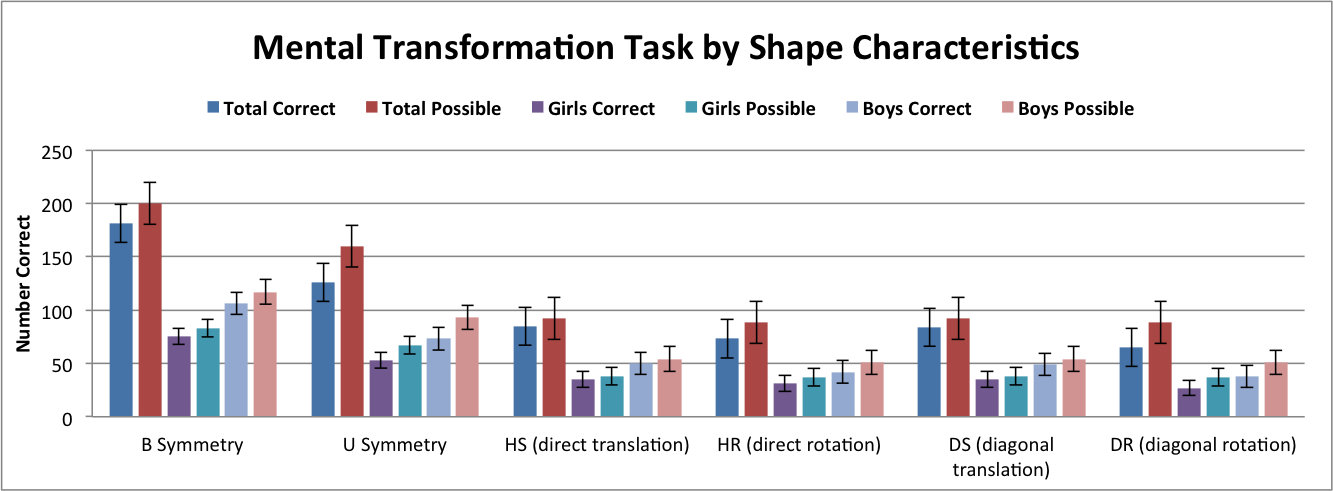
\includegraphics[width=.9\linewidth]{images/mttShape}
\end{center}
\caption{A view of the Mental Transformation Task results, broken out by
symmetry type (B = bilateral, U = unilateral) and rotation or translation type
performed on the shape being transformed.}
\label{mttbreakdown}
\end{figure}

Overall, subjects performed very well on the Mental Transformation Task,
correctly responding to 614 of 720 questions (a little over 85\%). Performance
was remarkably equal across genders, with girls correct on 256 of 300 (85.3\%)
and boys on 358 of 420 (85.2\%). Accordingly, we found no sigificant difference
in gendered responses across any symmetry or translation type - girls and boys
succeeded and struggled on the same sorts of tasks. Bilateral symmetry was
significantly easier than unilateral, with over 90\% of bilateral tasks and only
78\% of unilateral tasks performed correctly. Rotation was more difficult than
translation, and diagonal transformations were more problematic than direct
ones. Hence, diagonal rotations scored the lowest (75\%), followed by direct
rotations (82\%), diagonal translations (91\%), and direct translations (93\%).

% \begin{table}[!ht] 
% \small
%     \caption[Mental Transformation Task by Shape Profile and
%     Translation Type]{Mental Transformation Task by Shape Profile and
%     Translation Type}
%     \begin{center}
%     \begin{tabular}{| c | c | c | c | c | c | c | c | } \hline 
%     $  $ & $Bilateral$ & $Unilateral$ & $Direct$ & $Direct$ & $Diagonal$ &
%     $Diagonal$ & $Total$ \\
%     & $Symmetry$ & $Symmetry$ & $Translation$ & $Rotation$ &
%     $Translation$ & $Rotation$ & $Correct$ \\ \hline
%     $Session 1$ & 109/120 & 57/80 & 54/60 & 34/40 & 56/60 & 22/40 & 166/200 \\
%     \hline 
%     $Girls$ & 43/48 & 23/32 & 22/24 & 13/16 & 23/24 & 8/16 & 66/80 \\ \hline
%     $ Boys $ & 66/72 & 34/48 & 32/36 & 21/24 & 33/36 & 14/24 & 100/120 \\ \hline
%     $ $ &  &  &  &  &  &  & \\ \hline
%     $Session 2$ & 72/80 & 69/80 & 31/32 & 39/48 & 28/32 & 43/48 & 141/160 \\
%     \hline 
%     $Girls$ & 32/35 & 30/35 & 13/14 & 18/21 & 12/14 & 19/21 & 62/70 \\ \hline
%     $Boys$ & 42/45 & 39/45 & 18/18 & 21/17 & 16/18 & 24/27 & 79/90 \\ \hline
%     $ $ &  &  &  &  &  &  & \\ \hline
%     $Combined$ & 181/200 & 126/160 & 85/92 & 73/88 & 84/92 & 65/88 & 307/360 \\
%     \hline 
%     $Girls$ & 75/83 & 53/67 & 35/38 & 31/37 & 35/38  & 27/37 & 256/300 \\ \hline
%     $Boys$ & 108/117 & 73/93 & 50/54 & 42/51 & 49/54 & 38/51 & 360/420 \\ \hline
% 	\end{tabular}
%    \\ \rule{0mm}{5mm}
% \end{center}
% \label{MTTbyShape}
% \end{table}

% \begin{table}[!ht] 
% \tiny
%     \caption[Mental Transformation Task
%     Performance Per User]{Mental Transformation Task Performance Per User.}
%     \begin{center}
%     \begin{tabular}{| c | c | c | c | c | c | c | c | c | c | c | c | c | c | c
%     | c | c | c | c | c | c |} \hline 
%     $User$ & 1 & 2 & 3 & 4 & 5 & 6 & 7 & 8 & 9 & 10 & 11 & 12 & 13 & 14 & 15 &
%     16 & 17 & 18 & 19 & 20 \\ \hline
%     $Set$ $1$ & 7 & 10 & 8 & 7 & 9 & 8 & 10 & 9 & 9 & 7 & 9 & 8 & 10 & 9 & 6 &
%     8 & 10 & 8 & 7 & 7 \\\hline 
%     $Set$ $2$ & 9 & 9 & 10 & 6 & 10 & - & 10 & 10 & 10 & 10 & 9 & 9 & - & 6 &
%     - & - & 10 & 8 & 5 & 10 \\ \hline 
%     $Total$ & 16 & 19 & 18  & 13  & 19 & - & 20  & 19 & 19  & 17 & 18  & 17  & - 
%     & 15 & - & - & 20 & 16 & 12 & 17\\ \hline 
%     $Change$ & +2 & -1 & +2 & -1 & +1 & - & 0 & +1 & +1 & +3 & 0 & +1 & - &
%     -3 & - & - & 0 & 0 & -2 & +3 \\ \hline
% 	\end{tabular}
%    \\ \rule{0mm}{5mm}
% \end{center}
% \label{MTTperUser}
% \end{table}

\begin{figure}[!ht]
\begin{center}
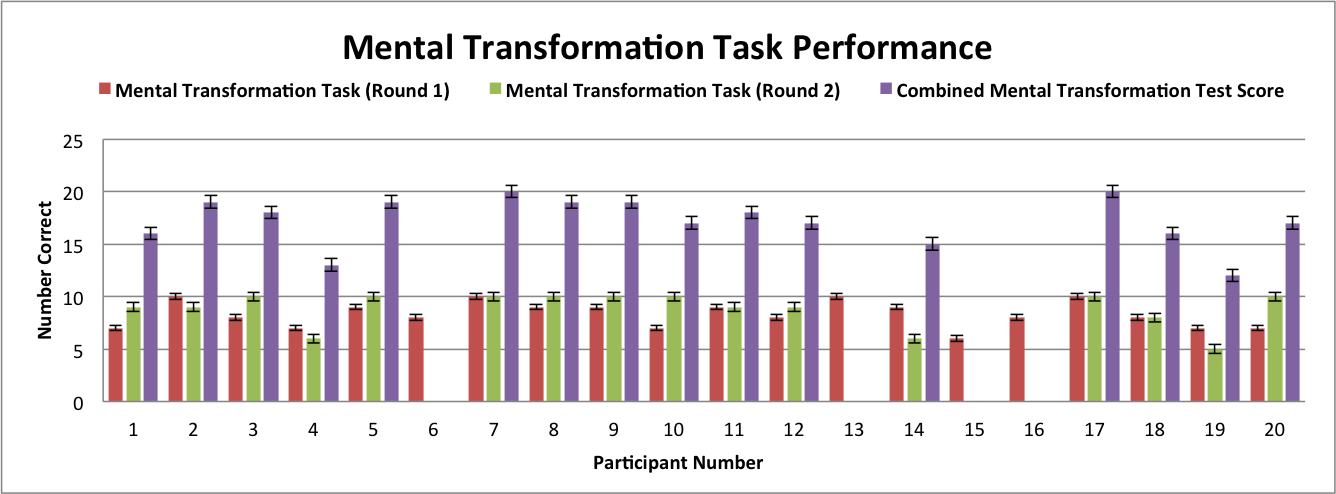
\includegraphics[width=.9\linewidth]{images/mttPerf}
\end{center}
\caption{Mental Transformation Task results, broken down by session and by
user.}
\label{MTTPerformance}
\end{figure}

Figure \ref{MTTPerformance} shows the Mental Transformation Task results broken
down into sessions by user. We observed a +7 net improvement in the second round
among the 16 users who participated in both sessions. Both girls and boys
improved in the second session, though girls improved by a greater percentage
when compared to boys - from 82.3\% to 88.6\% while boys improved from 83.3\% to
87.7\%, a 2\% greater improvement among girls. Four users did worse on the
second set of tasks, four did the same, and eight improved; the greatest change
in both directions was +/- 3. There was a no real correlation between
improvement between sessions (or lack thereof) and modeling performance overall
($r = .20, $ $p < .5$), nor was there a real correlation between improvement on
the Mental Transformation Task and improvement in modeling score from session 1
to session 2 ($r=-.20,$ $p <.5$), suggesting that the \emph{change} between
sessions on the spatial reasoning test and modeling performance are mildly
related, if at all.

\subsubsection{Speech and Gesture Coding Results}

During the modeling exercises, if a subject believed (correctly or not) that
they had successfully modeled a shape, the facilitator asked the subject to
describe the modeling strategy they used to arrive at their answer. During these
explanations, video recordings were analyzed for five types of speech and
gesture behaviors: those referring to movement, to the perceptual whole of the
shape being modeled, to a perceptual feature of the shape being model, as well
as behaviors that were vague or unintelligible, and those that did not fit into
any of the above categories (labeled as ``other'' - a more detailed description
is available in the procedure section above). A given strategy was only recorded
once per modeling task, but multiple strategies per explanation occurred often
and were recorded (as was also the case in \cite{ehrlich2006importance}). The
table below breaks down the numbers and types of speech and gesture observed
over the two sessions; as such, we only report on the 16 subjects who completed
both sessions. For further insight into how some of the modeling strategies were
expressed by the users as well as the associated coding and gesture
observations, we have compiled a set of excerpts in Appendix B. These excerpts
contain quotes from users while explaining their modeling strategy, the observed
gestures that occurred during the spoken explanation, and the speech and gesture
codes generated from those expressions.

% \begin{table}[!ht] 
% \tiny
%     \caption[Session 1 Gesture and Speech Observations]{Gesture and
%     Speech Observations over both sessions.}
%     \begin{center}
%     \begin{tabular}{| c | c | c | c | c | c | c | c | c | c | c | c | c | c | c
%     |} \hline
%     User & G.M & G.PW & G.PF & G.V & G.O & G Tot. & S.M & S.PW & S.PF & S.V &
%     S.O & S Tot. & G Tot. + & No. \\   
%     & & & & & & & & & & & & & S Tot. & Corr. \\ \hline
%     1 &4 &0 &8 &7 &0 &19 &4 &3 &7 &13 &4 &31 &50 &20 \\ \hline
%     2 &10 &1 &10 &6 &0 &27 &7 &7 &9 &6 &2 &31 &58 &14  \\ \hline
%     3 &1 &0 &9 &1 &0 &11 &4 &2 &11 &4 &0 &21 &32 &9  \\ \hline
%     4 &0 &0 &5 &9 &0 &14 &1 &7 &12 &9 &2 &31 &45 &9  \\ \hline
%     5 &6 &0 &11 &5 &0 &22 &8 &2 &11 &6 &4 &31 &53 &11  \\ \hline
%     7 &4 &0 &15 &6 &0 &25 &6 &3 &15 &2 &12 &38 &63 &23  \\ \hline
%     8 &1 &0 &2 &4 &0 &7 &1 &0 &2 &4 &0 &7 &14 &12  \\ \hline
%     9 &4 &2 &3 &10 &0 &19 &10 &6 &4 &8 &1 &29 &48 &11  \\ \hline
%     10 &10 &4 &19 &8 &2 &43 &5 &9 &19 &6 &4 &43 &86 &22  \\ \hline
%     11 &11 &2 &15 &5 &1 &34 &8 &3 &16 &5 &7 &39 &73 &21  \\ \hline
%     12 &6 &0 &10 &8 &0 &24 &5 &4 &7 &10 &3 &29 &53 &11  \\ \hline
%     14 &4 &1 &8 &7 &0 &20 &6 &3 &6 &7 &4 &26 &46 &6  \\ \hline
%     17 &16 &2 &23 &6 &0 &47 &14 &12 &22 &0 &7 &55 &102 &20  \\ \hline
%     18 &12 &1 &19 &2 &0 &34 &13 &3 &22 &2 &10 &50 &84 &20  \\ \hline
%     19 &17 &0 &14 &7 &2 &40 &13 &2 &14 &16 &3 &48 &88 &7  \\ \hline
%     20 &7 &0 &9 &9 &2 &27 &2 &2 &9 &6 &7 &26 &53 &5  \\ \hline
% 	\end{tabular}
%    \\ \rule{0mm}{5mm}
% \end{center}
% \label{MTTperUser}
% \end{table}


\begin{table}[!ht] 
\small
    \caption[Gesture and Speech Observations]{Gesture and Speech
    Observations over both sessions. Numbers in this table exclude the
    totals from the three subjects who finished the first session but not the
    second. \\ G = Gesture, S = Speech, .M = Movement, .PW = Perceptual Whole,
    .PF = Perceptual Feature, .V = Vague, .O = Other.}
    \begin{center}
    \begin{tabular}{| c | c | c | c | c | c | c | c | c | c | c |} \hline
	& $Total$ & & $PopCAD$ & $SnapCAD$ & & $Girls$ & $Boys$ & & $Session$ $1$ &
	$Session$ $2$\\ \hline 
	$G.M$ &113 & &62 &51 & &73 &40 & &39 &74 \\ \hline
	$G.PW$ &13 & &8 &5 & &8 &5 & &9 & 4 \\ \hline
	$G.PF$ &180 & &102 &78 & &96 &84& &93 &87 \\ \hline
	$G.V$ &100 & &50 &50 & &42 &58& &34 & 66 \\ \hline
	$G.O$ &7 & &4 &3 & &6 &1& &4 & 3\\ \hline
	 & & & & & & & & & &\\ \hline
	$S.M$ &107 & &64 &43 & &55 &52& &46 & 61\\ \hline
	$S.PW$ &68 & &39 &29 & &35 &33& & 38& 30 \\ \hline
	$S.PF$ &186 & &103 &83 & &97 &89 & &101 &85 \\ \hline
	$S.V$ &104 & &55 &49 & &40 &64 & &32 &72 \\ \hline
	$S.O$ &70 & &35 &35 & &33 &37 & & 18 & 52 \\ \hline
	 & & & & & & & & & & \\ \hline
	$Gesture$ &413 & &226 &187 & &225 &188& &179 & 234 \\ \hline
	$Speech$ &535 & &296 &239 & &260 &275 & & 235& 300\\ \hline
	$Combined$ &948 & &522 &426 & &485 &463& & 414& 534 \\ \hline
	\end{tabular}
   \\ \rule{0mm}{5mm}
\end{center}
\label{MTTperUser}
\end{table}

Table \ref{MTTperUser} shows the total number of gesture and speech types we
recorded, as well as how they were split between each devices, genders, and
sessions. The most common gesture and speech types (by a significant margin)
were about specific perceptual features of the models, those relating to
movement came next, followed closely by vague gestures and speech.
The other two categories, perceptual whole and ``other'' strategies, were barely
represented in gesture - they were far more common in speech, but still ranked
as the least frequently recorded. Many users explained their modeling strategy
by doing a ``step-by-step'' recounting of their process that referred at each
step to the part of the shape they were modeling at that point. For example, it
was common for a subject to point to a segment of the model and say (for
instance), ``and then I put a point here, for this part\ldots'', generating
perceptual feature scores in both gesture and speech for nearly every
explanation they gave. Movement was often explained along the same lines (though
less frequently), often with subject using specific words that indicate motion
(e.g. ``then I move over here'', ``I had to go up here, then follow the path
back down again'') while simultaneously motioning along the directions they were
indicating. Figure \ref{gestureSeries} shows a series of six still shots taken
from the video that depict (as best as possible in a single frame) various
gestures made during a single explanation of a modeling task strategy.

\begin{figure}[!ht]
\begin{center}$
\begin{array}{ccc}
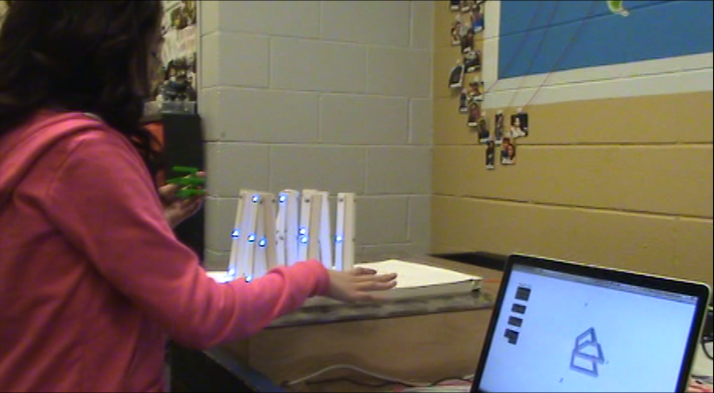
\includegraphics[width=.3\linewidth]{images/g1}&
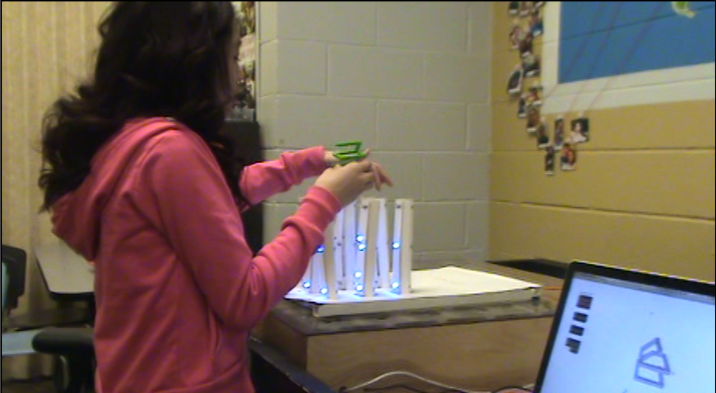
\includegraphics[width=.3\linewidth]{images/g2}&
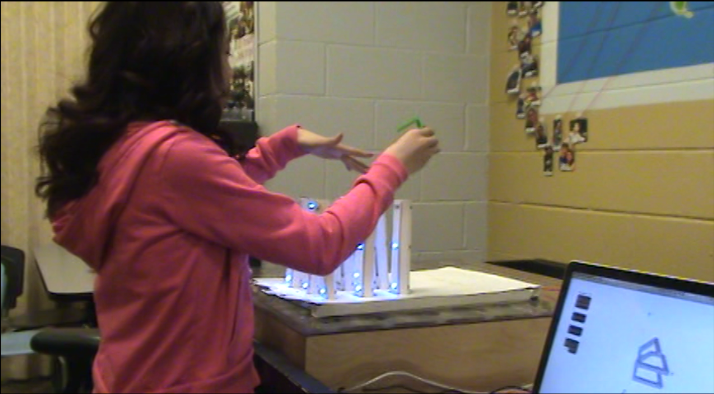
\includegraphics[width=.3\linewidth]{images/g3}\\
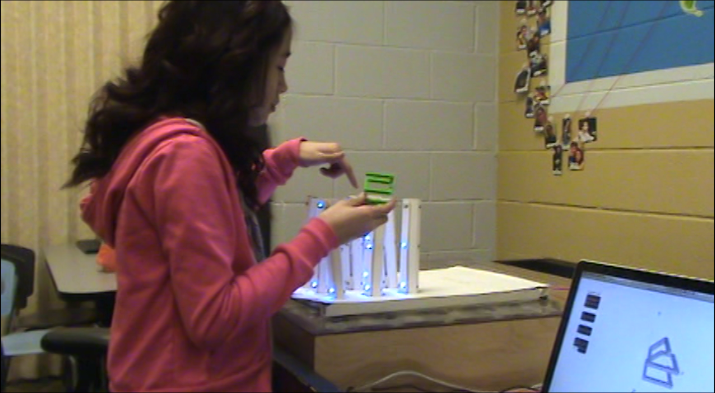
\includegraphics[width=.3\linewidth]{images/g4}&
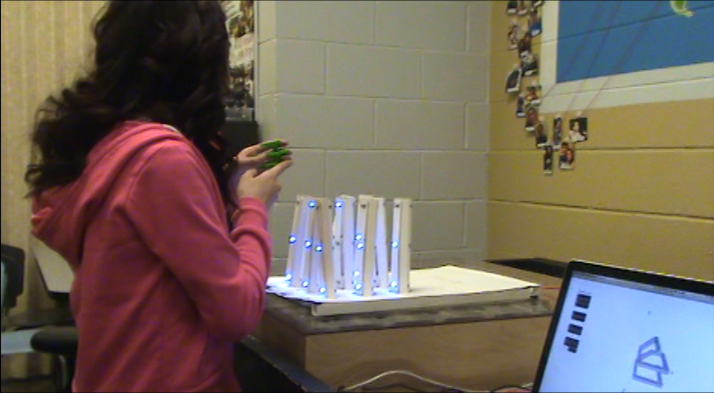
\includegraphics[width=.3\linewidth]{images/g5}&
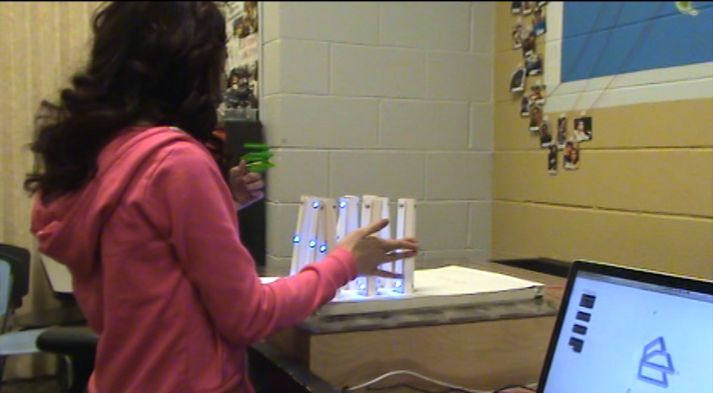
\includegraphics[width=.3\linewidth]{images/g6} \\
\end{array}$
\end{center}
\caption{A series of screen grabs from the video recording showing various
gestures from a user explaining her modeling strategy on one of the modeling
tasks.}
\label{gestureSeries}
\end{figure}


Interestingly, even without accounting for the difference in number of subjects,
girls ``out-gestured'' the boys overall (225 to 188), and in every category
\emph{except} for vague gestures, where boys were vague in describing their
strategies 24 more times over the course of the study. Speech types were more
gender-balanced, with the final tally being 260 for girls and 275 for boys,
however seeing as boys had more participants in both sessions of the study, the
speech-per-participant count actually favors the girls as well. The PopCAD
interface produced more gestures (226 to 187) and speech (296 to 239) than the
SnapCAD, a finding mitigated somewhat by the fact that users modeled so poorly
on the SnapCAD in the first round and therefore did not arrive at a point where
a modeling strategy could be explained. If we isolate the second round only,
where the performance breakdown was much more even (62 to 54 in favor of
PopCAD), then SnapCAD actually produced more gestures (124 to 110) and more
speech elements (159 to 141). 

Perhaps the most curious data from Table \ref{MTTperUser} is the big increase in
both gesture and speech from round one to round two of the study. Even with
three less participants in round two, overall instances of gestures increased
from round one by 55 (179 to 234, a 31\% increase), and speech instances
increased by 65 (235 to 300, a 28\% increase), yet the overall modeling
performance only increased by 5\% in round two. A bit of a closer look at the
types of gesture and speech gives a plausible explanation: in both gesture and
speech, the number of \emph{vague} indications rose dramatically (+32 for
gesture, +40 for speech), while the number of perceptual feature indications
dropped in both cases (-6 for gesture, -16 for speech). If we look at Figures
\ref{gesturebreakdown} and \ref{speechbreakdown} these numbers start to make
more sense.

\begin{figure}[!ht]
\begin{center}
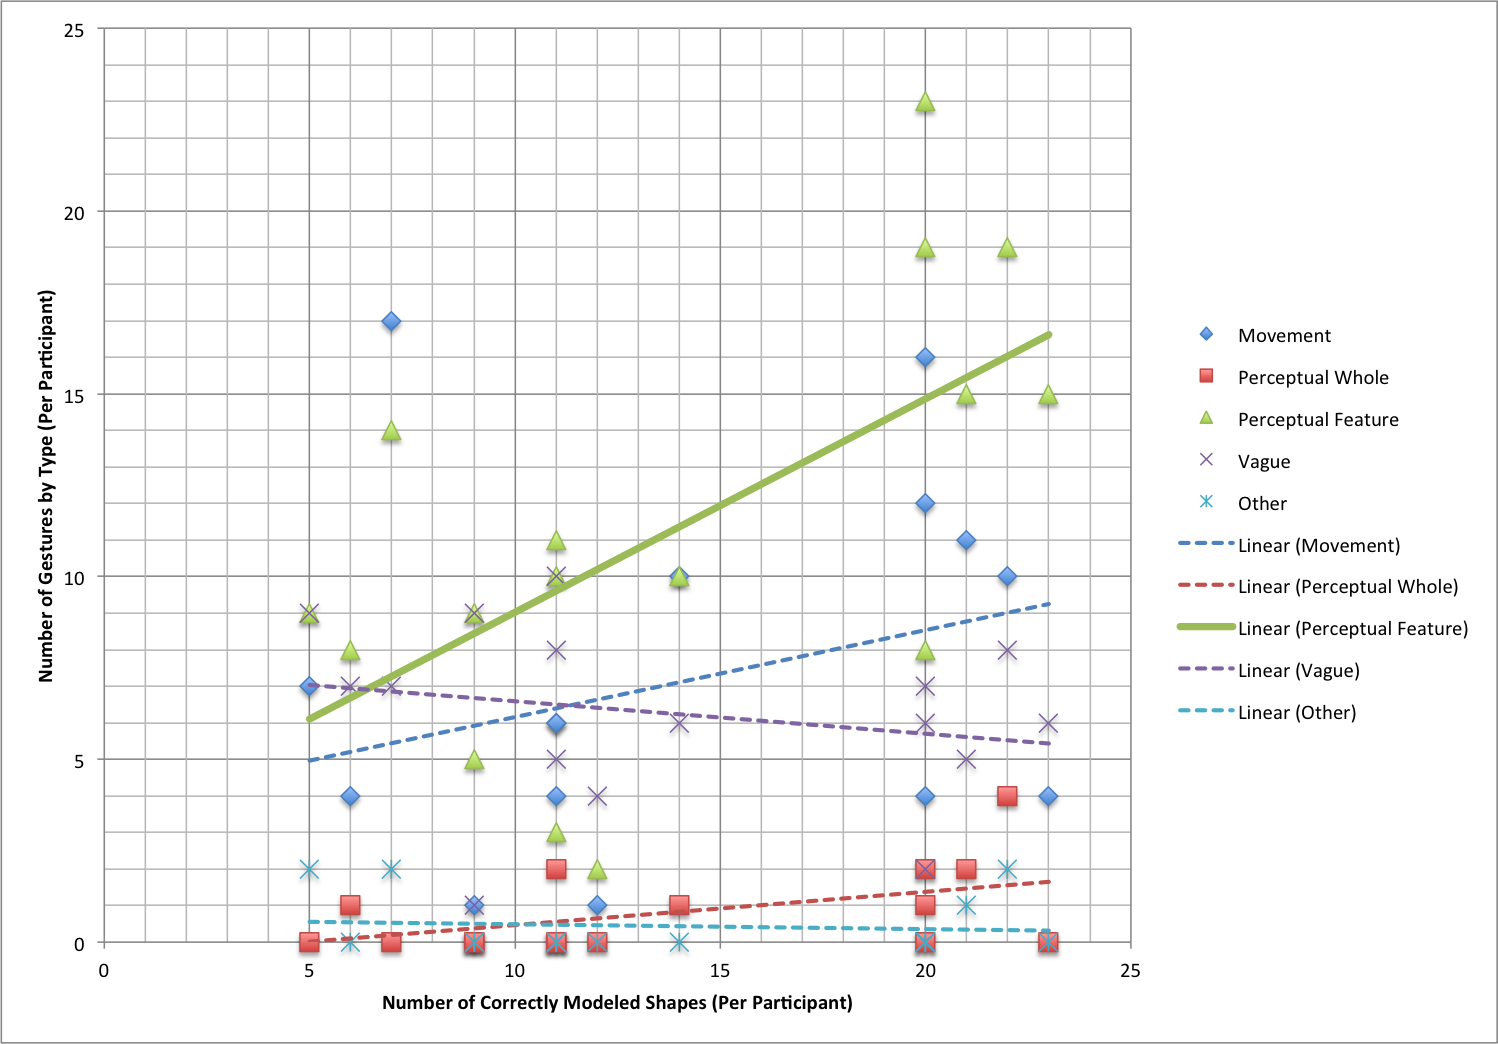
\includegraphics[width=.85\linewidth]{images/gestureGraph}
\end{center}
\caption{A plot of the five types of gestures we coded (movement, perceptual
whole, perceptual feature, vague, and other) over the number of correctly
modeled shapes. The slope of the lines indicate the strength of correlation
between each gesture type and overall modeling performance.}
\label{gesturebreakdown}
\end{figure}

Figure \ref{gesturebreakdown} shows a plot of the number and kind of gestures
produced by a user over the number of shapes they modeled correctly over the two
rounds of the study.\footnote{Data from the three users who dropped out of the
study has been omitted from this graph as well as Figure \ref{speechbreakdown}}
The lines associated with each scatter plot shows the strength of the
correlation between instances of that gesture type and modeling performance; the
steeper the positive slope, the higher the positive correlation and vice versa.
As we can see from the graph, three of the conditions have positive slopes
(perceptual feature, movement, and perceptual whole), while two have negative
slopes (vague and other). By far the strongest positive correlation\footnote{All
correlation calculations were done using Pearson's Correlation Coeffcient.} is
between perceptual feature gesturing and modeling performance ($r = .61,$ $p <
.025$), while vague gesturing has a weak negative correlation ($r = -.22,$ $p <
.5$). Going back to our earlier table, then, the sharp uptick in vague gestures
and mild decline of perceptual features may help to explain why such an increase
in gesturing did not result in a similar upswing in modeling performance.


\begin{figure}[!ht]
\begin{center}
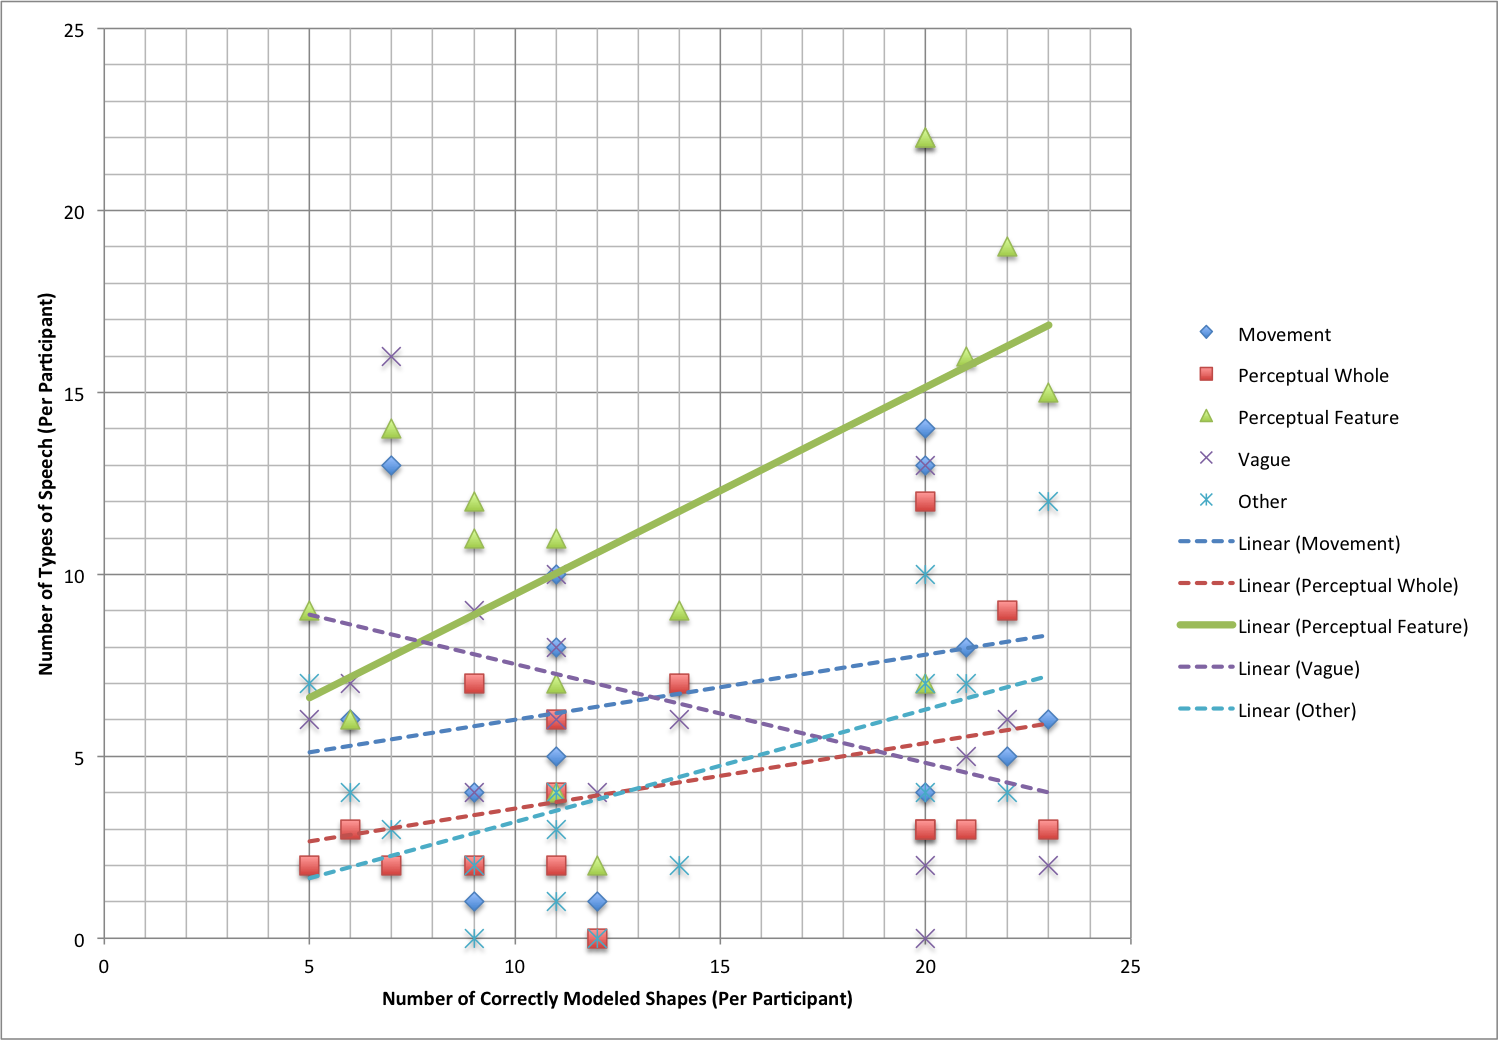
\includegraphics[width=.85\linewidth]{images/speechGraph}
\end{center}
\caption{A plot of the five types of speech we coded (movement, perceptual
whole, perceptual feature, vague, and other) over the number of correctly
modeled shapes. The slope of the lines indicate the strength of correlation
between each speech type and overall modeling performance.}
\label{speechbreakdown}
\end{figure}

One might expect that correlation patterns would be similar between gestures and
speech of the same type (e.g. instances of movement in gesture would be as
correlated to modeling performance as instances of movement in speech), and
while we did find some similarities, some surprising differences appeared as
well. Speaking about perceptual features was (as with gesturing) the most highly
correlated type to modeling success ($r = .58,$ $p < .025$), but where gestures
marked as ``other'' had a very weak negative correlation, ``other'' categories
of speech were second most \emph{highly} correlated with modeling aptitude ($r
=. 56,$ $p < .025$) - nearly as much as utterances on perceptual features. Part
of this explanation lies in the frequency discrepancy between ``other'' gestures,
of which there were only seven, and ``other'' speech utterances, of which there
were ten times more (70). The other (pardon the pun) part of the explanation
lies in the fact that we have many more words with specific meanings than
gestures that are precisely defined, so (for example) explanations referring to
looking at the software itself (e.g., ``I looked at the screen and it looked
like it''), or reasoning about the nature of how the mode works (e.g., ``Since
it was path I knew it would work''), or internal operations (e.g., ``I just
look at it and see it''), are harder to perceive in gesture. A possible relation
to the potential for specificity in speech lies in the stronger observed
negative correlation between modeling ability and speech marked as vague ($r=
-.41,$ $p < .25$), compared to gestures marked as vague ($r=-.22,$ $p < .5$),
indicating (perhaps) that a failure to speak specifically (given more abundant
options) is more harmful than a similar failure when gesturing.


\subsection{Observations}

A few notes on the above findings are worth making here. Broadly speaking, the
study indicated many positive outcomes: overall modeling ability went up while
average modeling time went down, the participants improved on every modeling
mode in the second session, there was a net positive performance on the second
mental transformation task when compared with the first, and participants were
generally engaged by the experience, which for most subjects was their first
computer-based 3D modeling experience. However, even though no user saw the same
device or shape twice, it is as yet unclear how much of the improvement might be
contributed to a ``practice effect''. Due to the ``drop-in'' nature of the user
study environment, the time between each single participants' sessions varied,
based on their attendance and availability (i.e., in some cases users had
homework or other activities to finish).

We observed some moderate correlations between types of speech and gesture and
modeling success, though not necessarily the kinds of correlations we might have
expected based on prior related studies. Nor were speech and gesture correlated
to modeling acumen in the same ways - some types of gesture were less effective
than their corresponding spoken elements, and vice versa. In some cases, the
results were observed were counter-intuitive - such as the anomaly in average
modeling times of subjects when using the minimal spanning tree mode, the fact
that boys performed worse during the second modeling session while girls
performed much better, and that some subjects performed worse on the second
mental transformation task, even though they were arguably ``primed'' by going
through the modeling exercises beforehand. Also unexpected is the sharp decline
in performance on the PopCAD device in the second session - over 10\% -
especially after such a high percentage in the first round and given more
``experienced'' users in the second session. Equally surprising, given a rather
unimpressive first round performance, is the sharp increase in modeling success
on the SnapCAD in the second round (a jump of 12\%), so much so that when
coupled with the decline in PopCAD performance, we may wonder on the possible
disparity between the groups in ``inherent'' ability for these kinds of tasks.
Another possibility is of course that the order in which subject encounter the
devices is more important than we had originally surmised - perhaps the users
who started with PopCAD did better on the SnapCAD (and overall) \emph{because}
they started with PopCAD. We examine these, as well as the relevance of age and
shape complexity on modeling ability, along with a deeper discussion of results
across all three studies in the following chapter.






% Given the massive development (both cognitively and physically) that occurs
% between the age extremes in our subject population (11 to 18), it would be
% tempting (and even logical) to assume that the older subjects would perform much
% better on the modeling tasks than their younger counterparts. However, we found
% a very modest correlation ($r = .39, p < .15$) between age and the number of
% correctly modeled shapes, suggesting it may play less of a role then we would
% have suspected. It is possible that the statistics are slightly misleading here
% - the subject population was weighted toward the younger end of the spectrum:
% the average age was 13.8, while median age was 13.5, and the mode was 12 years
% old. Meaning the few older participants would have had to perform impossibly
% brilliantly (i.e., higher than the highest possible score) for a strong age to
% performance correlation to show up.
% 
% Popcad first avg age: 14
% snapcad first : 13.75
% 
% 
% In order to attempt to judge each shape's complexity, we sought out a
% previously-defined set of criteria by which to judge ``complexity''. As it turns
% out, there is a long and thorough discussion of complexity in relation to
% \emph{two-dimensional} shapes, starting seemingly with Fred Attneave and Malcolm
% Arnoult\cite{attneave1956quantitative}\cite{attneave1957physical} in the mid
% 1950's, who define methods of generating random two-dimensional shapes and
% examine their physical characteristics in relation to their judged complexity.
% As it turns out (in \cite{attneave1957physical} as well as others' follow-up
% work) the ``Number of Turns'' in the shape was responsible for significant
% amount (nearly 80\% in Attneave's study) of the preceived complexity of a shape.
% ``Number of Turns'' is defined as, ``the number of maxima (regardless of sign)
% in one cycle of the function relating curvature to distance along the contour.
% This function is a series of spikes for any angular shape, and a step-function
% for any curved shape\ldots'' (see pp. 226 of the aforementioned article).
% Symmetry, angular variability, and squared perimeter over area also had some
% affect.
% 
% However, as it seems unclear to us how one might adapt a ``Number of Turns''
% rating to a true \emph{three dimensional} model. Although many studies claim to
% have studied complexity in relation to mental transformation tasks, starting
% with Shepard and Metzler\cite{shepard1971mental}, who instead used perspective
% line drawings, not actual physical models. This had an advantage for the types
% of mental rotation tasks they were performing (recognition of matching pairs),
% and similarly set off a wave of studies using the same (or similar) ``faux 3D''
% stimuli\cite{metzler1974transformational}\cite{shepard1988mental}\cite{vandenberg1978mental}.
% 
% All of which leads us to determine (as best we way) the complexity of the shapes
% we presented in the study, as a way of teasing out any correlation between
% complexity and performance. In lieu of attempting an exact number of turns
% estimate, we included three criteria: (a) the minimum number of lights necessary
% to guarantee the correct shape,\footnote{In minimal spanning tree models where a
% placement of lights results in several possible correct formations, only one of
% which is the desired shape, we add points necessary to ``force'' the correct
% representation.} (b) the number of faces (for convex hull models only), the
% number of line segments (for path models only), or the number of distinct
% branches (for tree models only), and (c) a symmetry score based on number of
% lines of symmetry, from 3 (indicating asymmetry) to 0 (indicating 3 or more
% lines of symmetry). The scaling for symmetry comes from the belief that
% indicators (a) and (b) above are more closely aligned with Attneave's ``number
% of turns'' metric (being highly correlated to perceived difficulty), while
% symmetry was much less correlated to complexity (although symmetry did still
% play a part), so we made the scale as low as possible so that it would weigh
% less on the overall complexity score of a model. So, for example, a regular
% octahedron would have 6 points, 8 faces, and a 0 symmetry score for an overall
% difficulty score of 14. The complexity score of each shape is shown in
% \ref{modelComplexity} next to the number of times it was modeled correctly. The
% shapes in each session were of course different, but are labeled the same in
% this table, indicating the order in which they were presented.
% 
% 
% 
% \begin{table}[!ht] 
% \small
%     \caption[Complexity of Models and Modeling Performance]{Complexity of Models
%     and Modeling Performance (CH = Convex Hull, P = Path, T = Minimal Spanning
%     Tree)}
%     \begin{center}
%     \begin{tabular}{| c | c | c | c | c | c | c | c | c | c | c | c | c | }
%     \hline $ $ & CH1 & CH2 & CH3 & CH4 & P1 & P2 & P3 & P4 & T1 & T2 & T3 & T4 \\
%    	\hline
%    	$Session$ $1$ & & & & & & & & & & & &  \\ \hline
%    	$Complexity$ $Score$ & 14 & 19 & 19 & 19 & 7 & 18 & 20 & 24 & 9 & 13 & 17 &
%    	17 \\ \hline 
%    	$Performance$ of 19 & 8 & 13 & 8 & 11 & 17 & 14 & 8 & 9 & 12 & 8 & 8 & 11 \\
%    	\hline 
%    	$Session$ $2$ & & & & & & & & & & & & \\ \hline
%    	$Complexity$ $Score$ & 12 & 20 & 15 & 13 & 14 & 14 & 18 & 17 & 21 & 17 & 16
%    	& 25 \\ \hline 
%    	$Performance$ of 16 & 7 & 9 & 11 & 11 & 11 & 13 & 8 & 12 & 7 & 11 & 7 & 9 \\
%    	\hline
%    	
% 	\end{tabular}
%    \\ \rule{0mm}{5mm}
% \end{center}
% \label{modelComplexity}
% \end{table}
% 
% 
% One might expect to see a strong negative correlation between a given model's
% complexity score and the number of subjects who were able to model it correctly,
% however the observed correlation (using Pearson's correlation coefficient) was
% only moderate: $r = -0.41, p < .05$ over both sessions.
% 
% 
% Levine and Goldin-Meadow's research found the highest correlation occurred
% between the number of movement gestures produced over the number of correct
% answers given. 
% 
% 
% 
% The process of modeling is different than that of shape matching - modeling is
% by necessity a series of step-by-step, piecemeal operations, whereby in a mental
% transformation task, it is possible both to look at specific features of a shape
% as well as receive a more holistic mental image of the shape at hand. This may
% account in part for the relative lack of correlation between movement gestures
% and performance when compared to \cite{ehrlich2006importance}. Instead, we found
% a much higher correlation between gestures relating to perceptual features of
% the shape and modeling performance. One might argue that by looking at
% perceptual features of the shape, one is mentally ``breaking apart'' the shape
% into discrete chunks that can be turned into an order of operations for
% successfully modeling a shape.
